% Options for packages loaded elsewhere
\PassOptionsToPackage{unicode}{hyperref}
\PassOptionsToPackage{hyphens}{url}
%
\documentclass[
  letterpaper,
]{book}

\usepackage{amsmath,amssymb}
\usepackage{lmodern}
\usepackage{iftex}
\ifPDFTeX
  \usepackage[T1]{fontenc}
  \usepackage[utf8]{inputenc}
  \usepackage{textcomp} % provide euro and other symbols
\else % if luatex or xetex
  \usepackage{unicode-math}
  \defaultfontfeatures{Scale=MatchLowercase}
  \defaultfontfeatures[\rmfamily]{Ligatures=TeX,Scale=1}
\fi
% Use upquote if available, for straight quotes in verbatim environments
\IfFileExists{upquote.sty}{\usepackage{upquote}}{}
\IfFileExists{microtype.sty}{% use microtype if available
  \usepackage[]{microtype}
  \UseMicrotypeSet[protrusion]{basicmath} % disable protrusion for tt fonts
}{}
\makeatletter
\@ifundefined{KOMAClassName}{% if non-KOMA class
  \IfFileExists{parskip.sty}{%
    \usepackage{parskip}
  }{% else
    \setlength{\parindent}{0pt}
    \setlength{\parskip}{6pt plus 2pt minus 1pt}}
}{% if KOMA class
  \KOMAoptions{parskip=half}}
\makeatother
\usepackage{xcolor}
\setlength{\emergencystretch}{3em} % prevent overfull lines
\setcounter{secnumdepth}{5}
% Make \paragraph and \subparagraph free-standing
\ifx\paragraph\undefined\else
  \let\oldparagraph\paragraph
  \renewcommand{\paragraph}[1]{\oldparagraph{#1}\mbox{}}
\fi
\ifx\subparagraph\undefined\else
  \let\oldsubparagraph\subparagraph
  \renewcommand{\subparagraph}[1]{\oldsubparagraph{#1}\mbox{}}
\fi

\usepackage{color}
\usepackage{fancyvrb}
\newcommand{\VerbBar}{|}
\newcommand{\VERB}{\Verb[commandchars=\\\{\}]}
\DefineVerbatimEnvironment{Highlighting}{Verbatim}{commandchars=\\\{\}}
% Add ',fontsize=\small' for more characters per line
\usepackage{framed}
\definecolor{shadecolor}{RGB}{241,243,245}
\newenvironment{Shaded}{\begin{snugshade}}{\end{snugshade}}
\newcommand{\AlertTok}[1]{\textcolor[rgb]{0.68,0.00,0.00}{#1}}
\newcommand{\AnnotationTok}[1]{\textcolor[rgb]{0.37,0.37,0.37}{#1}}
\newcommand{\AttributeTok}[1]{\textcolor[rgb]{0.40,0.45,0.13}{#1}}
\newcommand{\BaseNTok}[1]{\textcolor[rgb]{0.68,0.00,0.00}{#1}}
\newcommand{\BuiltInTok}[1]{\textcolor[rgb]{0.00,0.23,0.31}{#1}}
\newcommand{\CharTok}[1]{\textcolor[rgb]{0.13,0.47,0.30}{#1}}
\newcommand{\CommentTok}[1]{\textcolor[rgb]{0.37,0.37,0.37}{#1}}
\newcommand{\CommentVarTok}[1]{\textcolor[rgb]{0.37,0.37,0.37}{\textit{#1}}}
\newcommand{\ConstantTok}[1]{\textcolor[rgb]{0.56,0.35,0.01}{#1}}
\newcommand{\ControlFlowTok}[1]{\textcolor[rgb]{0.00,0.23,0.31}{#1}}
\newcommand{\DataTypeTok}[1]{\textcolor[rgb]{0.68,0.00,0.00}{#1}}
\newcommand{\DecValTok}[1]{\textcolor[rgb]{0.68,0.00,0.00}{#1}}
\newcommand{\DocumentationTok}[1]{\textcolor[rgb]{0.37,0.37,0.37}{\textit{#1}}}
\newcommand{\ErrorTok}[1]{\textcolor[rgb]{0.68,0.00,0.00}{#1}}
\newcommand{\ExtensionTok}[1]{\textcolor[rgb]{0.00,0.23,0.31}{#1}}
\newcommand{\FloatTok}[1]{\textcolor[rgb]{0.68,0.00,0.00}{#1}}
\newcommand{\FunctionTok}[1]{\textcolor[rgb]{0.28,0.35,0.67}{#1}}
\newcommand{\ImportTok}[1]{\textcolor[rgb]{0.00,0.46,0.62}{#1}}
\newcommand{\InformationTok}[1]{\textcolor[rgb]{0.37,0.37,0.37}{#1}}
\newcommand{\KeywordTok}[1]{\textcolor[rgb]{0.00,0.23,0.31}{#1}}
\newcommand{\NormalTok}[1]{\textcolor[rgb]{0.00,0.23,0.31}{#1}}
\newcommand{\OperatorTok}[1]{\textcolor[rgb]{0.37,0.37,0.37}{#1}}
\newcommand{\OtherTok}[1]{\textcolor[rgb]{0.00,0.23,0.31}{#1}}
\newcommand{\PreprocessorTok}[1]{\textcolor[rgb]{0.68,0.00,0.00}{#1}}
\newcommand{\RegionMarkerTok}[1]{\textcolor[rgb]{0.00,0.23,0.31}{#1}}
\newcommand{\SpecialCharTok}[1]{\textcolor[rgb]{0.37,0.37,0.37}{#1}}
\newcommand{\SpecialStringTok}[1]{\textcolor[rgb]{0.13,0.47,0.30}{#1}}
\newcommand{\StringTok}[1]{\textcolor[rgb]{0.13,0.47,0.30}{#1}}
\newcommand{\VariableTok}[1]{\textcolor[rgb]{0.07,0.07,0.07}{#1}}
\newcommand{\VerbatimStringTok}[1]{\textcolor[rgb]{0.13,0.47,0.30}{#1}}
\newcommand{\WarningTok}[1]{\textcolor[rgb]{0.37,0.37,0.37}{\textit{#1}}}

\providecommand{\tightlist}{%
  \setlength{\itemsep}{0pt}\setlength{\parskip}{0pt}}\usepackage{longtable,booktabs,array}
\usepackage{calc} % for calculating minipage widths
% Correct order of tables after \paragraph or \subparagraph
\usepackage{etoolbox}
\makeatletter
\patchcmd\longtable{\par}{\if@noskipsec\mbox{}\fi\par}{}{}
\makeatother
% Allow footnotes in longtable head/foot
\IfFileExists{footnotehyper.sty}{\usepackage{footnotehyper}}{\usepackage{footnote}}
\makesavenoteenv{longtable}
\usepackage{graphicx}
\makeatletter
\def\maxwidth{\ifdim\Gin@nat@width>\linewidth\linewidth\else\Gin@nat@width\fi}
\def\maxheight{\ifdim\Gin@nat@height>\textheight\textheight\else\Gin@nat@height\fi}
\makeatother
% Scale images if necessary, so that they will not overflow the page
% margins by default, and it is still possible to overwrite the defaults
% using explicit options in \includegraphics[width, height, ...]{}
\setkeys{Gin}{width=\maxwidth,height=\maxheight,keepaspectratio}
% Set default figure placement to htbp
\makeatletter
\def\fps@figure{htbp}
\makeatother
\newlength{\cslhangindent}
\setlength{\cslhangindent}{1.5em}
\newlength{\csllabelwidth}
\setlength{\csllabelwidth}{3em}
\newlength{\cslentryspacingunit} % times entry-spacing
\setlength{\cslentryspacingunit}{\parskip}
\newenvironment{CSLReferences}[2] % #1 hanging-ident, #2 entry spacing
 {% don't indent paragraphs
  \setlength{\parindent}{0pt}
  % turn on hanging indent if param 1 is 1
  \ifodd #1
  \let\oldpar\par
  \def\par{\hangindent=\cslhangindent\oldpar}
  \fi
  % set entry spacing
  \setlength{\parskip}{#2\cslentryspacingunit}
 }%
 {}
\usepackage{calc}
\newcommand{\CSLBlock}[1]{#1\hfill\break}
\newcommand{\CSLLeftMargin}[1]{\parbox[t]{\csllabelwidth}{#1}}
\newcommand{\CSLRightInline}[1]{\parbox[t]{\linewidth - \csllabelwidth}{#1}\break}
\newcommand{\CSLIndent}[1]{\hspace{\cslhangindent}#1}

%
% ------ Initial setup defs  ------
%
\topmargin=-0.3in
\textheight=9.2in
\oddsidemargin=-0.2in
\evensidemargin=0.0in
\textwidth=6.90in
\parindent=30pt
\parskip=3pt
\headheight=15pt
\reversemarginpar
\marginparwidth=.75in
%
%
\setcounter{secnumdepth}{2}
\renewcommand{\theequation}{\thesection.\arabic{equation}}
\renewcommand{\thesubsection}{}
\newcommand{\doublesp}{\renewcommand{\baselinestretch}{2.0}}
\newcommand{\mediumsp}{\renewcommand{\baselinestretch}{1.6}}
\newcommand{\singlesp}{\renewcommand{\baselinestretch}{1.0}}
% 
\pagestyle{myheadings}
\thispagestyle{empty}
\markright{\today}
\newlength{\figlen}
\setlength{\figlen}{3.7in}
\renewcommand{\labelitemi}{$\bullet$}
\renewcommand{\labelitemii}{$\cdot$}

\makeatletter
\@ifpackageloaded{tcolorbox}{}{\usepackage[many]{tcolorbox}}
\@ifpackageloaded{fontawesome5}{}{\usepackage{fontawesome5}}
\definecolor{quarto-callout-color}{HTML}{909090}
\definecolor{quarto-callout-note-color}{HTML}{0758E5}
\definecolor{quarto-callout-important-color}{HTML}{CC1914}
\definecolor{quarto-callout-warning-color}{HTML}{EB9113}
\definecolor{quarto-callout-tip-color}{HTML}{00A047}
\definecolor{quarto-callout-caution-color}{HTML}{FC5300}
\definecolor{quarto-callout-color-frame}{HTML}{acacac}
\definecolor{quarto-callout-note-color-frame}{HTML}{4582ec}
\definecolor{quarto-callout-important-color-frame}{HTML}{d9534f}
\definecolor{quarto-callout-warning-color-frame}{HTML}{f0ad4e}
\definecolor{quarto-callout-tip-color-frame}{HTML}{02b875}
\definecolor{quarto-callout-caution-color-frame}{HTML}{fd7e14}
\makeatother
\makeatletter
\makeatother
\makeatletter
\@ifpackageloaded{bookmark}{}{\usepackage{bookmark}}
\makeatother
\makeatletter
\@ifpackageloaded{caption}{}{\usepackage{caption}}
\AtBeginDocument{%
\ifdefined\contentsname
  \renewcommand*\contentsname{Table of contents}
\else
  \newcommand\contentsname{Table of contents}
\fi
\ifdefined\listfigurename
  \renewcommand*\listfigurename{List of Figures}
\else
  \newcommand\listfigurename{List of Figures}
\fi
\ifdefined\listtablename
  \renewcommand*\listtablename{List of Tables}
\else
  \newcommand\listtablename{List of Tables}
\fi
\ifdefined\figurename
  \renewcommand*\figurename{Figure}
\else
  \newcommand\figurename{Figure}
\fi
\ifdefined\tablename
  \renewcommand*\tablename{Table}
\else
  \newcommand\tablename{Table}
\fi
}
\@ifpackageloaded{float}{}{\usepackage{float}}
\floatstyle{ruled}
\@ifundefined{c@chapter}{\newfloat{codelisting}{h}{lop}}{\newfloat{codelisting}{h}{lop}[chapter]}
\floatname{codelisting}{Listing}
\newcommand*\listoflistings{\listof{codelisting}{List of Listings}}
\makeatother
\makeatletter
\@ifpackageloaded{caption}{}{\usepackage{caption}}
\@ifpackageloaded{subcaption}{}{\usepackage{subcaption}}
\makeatother
\makeatletter
\@ifpackageloaded{tcolorbox}{}{\usepackage[many]{tcolorbox}}
\makeatother
\makeatletter
\@ifundefined{shadecolor}{\definecolor{shadecolor}{rgb}{.97, .97, .97}}
\makeatother
\makeatletter
\makeatother
\ifLuaTeX
  \usepackage{selnolig}  % disable illegal ligatures
\fi
\IfFileExists{bookmark.sty}{\usepackage{bookmark}}{\usepackage{hyperref}}
\IfFileExists{xurl.sty}{\usepackage{xurl}}{} % add URL line breaks if available
\urlstyle{same} % disable monospaced font for URLs
\hypersetup{
  pdftitle={Comparing Treatments for Amblyopia with a Synaptic Plasticity Model},
  pdfauthor={Brian S. Blais},
  hidelinks,
  pdfcreator={LaTeX via pandoc}}

\title{Comparing Treatments for Amblyopia with a Synaptic Plasticity
Model}
\usepackage{etoolbox}
\makeatletter
\providecommand{\subtitle}[1]{% add subtitle to \maketitle
  \apptocmd{\@title}{\par {\large #1 \par}}{}{}
}
\makeatother
\subtitle{.}
\author{Brian S. Blais}
\date{10/20/22}

\begin{document}
\frontmatter
\maketitle
\ifdefined\Shaded\renewenvironment{Shaded}{\begin{tcolorbox}[interior hidden, borderline west={3pt}{0pt}{shadecolor}, breakable, enhanced, sharp corners, boxrule=0pt, frame hidden]}{\end{tcolorbox}}\fi

\renewcommand*\contentsname{Table of contents}
{
\setcounter{tocdepth}{2}
\tableofcontents
}
\mainmatter
\bookmarksetup{startatroot}

\hypertarget{preface}{%
\chapter*{Preface}\label{preface}}
\addcontentsline{toc}{chapter}{Preface}

These notes are produced with Quarto.
(\url{https://quarto.org/docs/books})

\hypertarget{software-installation}{%
\section*{Software Installation}\label{software-installation}}
\addcontentsline{toc}{section}{Software Installation}

The software is Python-based with parts written in Cython.

\begin{itemize}
\tightlist
\item
  Download the Anaconda Distribution of Python:
\end{itemize}

https://www.anaconda.com/products/individual\#downloads.

\begin{itemize}
\tightlist
\item
  Download and extract the \emph{PlasticNet} package at:
\end{itemize}

https://github.com/bblais/Plasticnet/archive/refs/heads/master.zip

\begin{itemize}
\tightlist
\item
  Run the script \texttt{install.py}
\end{itemize}

\hypertarget{printable-versions}{%
\section*{Printable Versions}\label{printable-versions}}
\addcontentsline{toc}{section}{Printable Versions}

Printable versions of this report can be found on the GitHub site for
this project,

\begin{itemize}
\tightlist
\item
  \href{https://github.com/bblais/Amblyopia-Simulation/raw/main/docs/Comparing-Treatments-for-Amblyopia-with-a-Synaptic-Plasticity-Model.docx}{Microsoft
  Word version}
\item
  \href{https://github.com/bblais/Amblyopia-Simulation/raw/main/docs/Comparing-Treatments-for-Amblyopia-with-a-Synaptic-Plasticity-Model.pdf}{PDF
  version}
\end{itemize}

\part{Introduction}

In this part we will explore the clinical basis for amblyopia and its
treatments. In the Chapter~\ref{sec-models-of-development} and
Chapter~\ref{sec-models-of-treatments} we will explore the models that
are used to describe the deficits from amblyopia and their treatment,
respectively.

\hypertarget{what-is-amblyopia}{%
\chapter{What is Amblyopia?}\label{what-is-amblyopia}}

Amblyopia is the most common cause of vision loss in children, caused by
refractive errors or misalignment of the eyes (Zárate and Tejedor 2007).

\begin{itemize}
\tightlist
\item
  Visual acuity
\item
  Contrast sensitivity
\item
  Color
\item
  Depth (Stereopsis)
\item
  Motion
\item
  Visual fields
\end{itemize}

\hypertarget{how-is-it-treated}{%
\section{How is it Treated?}\label{how-is-it-treated}}

The current primary treatment is described in the \emph{Amblyopia
Preferred Practice Method} (D. K. Wallace et al. 2018). Treatments are
divided into two broad categories, monocular and binocular treatments.
Monocular treatments produce a competition between the two eyes by
treating only the fellow eye to that the amblyopic eye recovers.
Binocular treatments seek to stimulate both eyes in such a way that
binocular mechanisms can produce a recovery in the amblyopic eye.

\hypertarget{monocular-treatments}{%
\subsection{Monocular Treatments}\label{monocular-treatments}}

The most common treatment includes

\begin{enumerate}
\def\labelenumi{\arabic{enumi}.}
\tightlist
\item
  the optical correction of significant refractive errors
\item
  patching the dominant eye which forces the visual input to come from
  only the amblyopic eye.
\end{enumerate}

Although patching is the most common method of treatment, other methods
are described including pharmacology and technology (Jonathan M. Holmes
et al. 2016b; Kelly et al. 2016; Jonathan M. Holmes et al. 2016a; Li et
al. 2015; Zárate and Tejedor 2007; Gao et al. 2018; Glaser et al. 2002).
These include,

\begin{enumerate}
\def\labelenumi{\arabic{enumi}.}
\setcounter{enumi}{2}
\tightlist
\item
  Pharmacological treatment with atropine drops in the fellow eye
\end{enumerate}

Each of these treatments only directly applies to the fellow eye and the
amblyopic eye is left untouched.

\hypertarget{binocular-treatments}{%
\subsection{Binocular Treatments}\label{binocular-treatments}}

There are some treatments which are administered to both eyes, making
them binocular treatments. The one that we will be addressing here use
virtual reality headsets(Xiao et al. 2020, 2022),

\begin{enumerate}
\def\labelenumi{\arabic{enumi}.}
\setcounter{enumi}{3}
\tightlist
\item
  Virtual reality input to both eyes, with contrast modification and/or
  dichoptic masks
\end{enumerate}

\hypertarget{mechanisms-for-amblyopia}{%
\section{Mechanisms for Amblyopia}\label{mechanisms-for-amblyopia}}

Since the unequal visual input to the brain can cause alterations in the
synaptic pathways leading to a disparity in ocular dominance (Birch
2013), it is important to understand the possible synaptic effects
amblyopia can produce and how potential treatments will either help or
hinder the recovery.

\part{Methods}

In this paper we use a specific model of neural plasticity, the BCM
model(Bienenstock, Cooper, and Munro 1982), to describe the dynamics of
the recovery from amblyopia under a number of treatment protocols.

\hypertarget{natural-image-input-environment}\NormalTok{matplotlib inline}
\ImportTok{from}\NormalTok{ input\_environment\_defs }\ImportTok{import} \OperatorTok{*}
\end{Highlighting}
\end{Shaded}

In order to approximate the visual system, we start with the following
basic properties of the retina, LGN and cortex. There are approximately
1000 photoreceptors feeding into 1 ganglion cell (Jeon, Strettoi, and
Masland 1998; Sterling, Freed, and Smith 1988). The retina/LGN responses
show a center-surround organization, but with a center diameter less
than 1\(^o\) (Hubel 1995)

We use natural scene stimuli for the simulated inputs to the visual
system. We start with images taken with a digital camera, with
dimensions 1200 pixels by 1600 pixels and 40\(^o\) by 60\(^o\)
real-world angular dimensions (Figure Figure~\ref{fig-orig}).
Photoreceptors have a logarithmic response to the stimulus, so we apply
the natural logarithm to the pixel values. Finally, we model the
ganglion responses using a 32x32 pixel center-surround
difference-of-Gaussians (DOG) filter to process the images, each pixel
representing one photoreceptor (Figure Figure~\ref{fig-logdog}). The
center-surround radius ratio used for the ganglion cell is 1:3, with
balanced excitatory and inhibitory regions and normalized Gaussian
profiles.

\begin{Shaded}
\begin{Highlighting}[]
\CommentTok{\# Make the original image files}
\NormalTok{make\_original\_image\_files()}

\end{Highlighting}
\end{Shaded}

\begin{Shaded}
\begin{Highlighting}[]
\NormalTok{fname}\OperatorTok{=}\StringTok{\textquotesingle{}asdf/bbsk081604\_all.asdf\textquotesingle{}}
\NormalTok{image\_data}\OperatorTok{=}\NormalTok{pi5.asdf\_load\_images(fname)}
\NormalTok{im}\OperatorTok{=}\NormalTok{[arr.astype(}\BuiltInTok{float}\NormalTok{)}\OperatorTok{*}\NormalTok{image\_data[}\StringTok{\textquotesingle{}im\_scale\_shift\textquotesingle{}}\NormalTok{][}\DecValTok{0}\NormalTok{]}\OperatorTok{+}
\NormalTok{        image\_data[}\StringTok{\textquotesingle{}im\_scale\_shift\textquotesingle{}}\NormalTok{][}\DecValTok{1}\NormalTok{] }\ControlFlowTok{for}\NormalTok{ arr }\KeywordTok{in}\NormalTok{ image\_data[}\StringTok{\textquotesingle{}im\textquotesingle{}}\NormalTok{]]}
\KeywordTok{del}\NormalTok{ image\_data}
\NormalTok{plt.figure(figsize}\OperatorTok{=}\NormalTok{(}\DecValTok{16}\NormalTok{,}\DecValTok{8}\NormalTok{))}
\ControlFlowTok{for}\NormalTok{ i }\KeywordTok{in} \BuiltInTok{range}\NormalTok{(}\DecValTok{6}\NormalTok{):}
\NormalTok{    plt.subplot(}\DecValTok{2}\NormalTok{,}\DecValTok{3}\NormalTok{,i}\OperatorTok{+}\DecValTok{1}\NormalTok{)}
\NormalTok{    plt.imshow(im[i],cmap}\OperatorTok{=}\NormalTok{plt.cm.gray)}
\NormalTok{    plt.axis(}\StringTok{\textquotesingle{}off\textquotesingle{}}\NormalTok{)}
\end{Highlighting}
\end{Shaded}

\begin{figure}[H]

{\centering 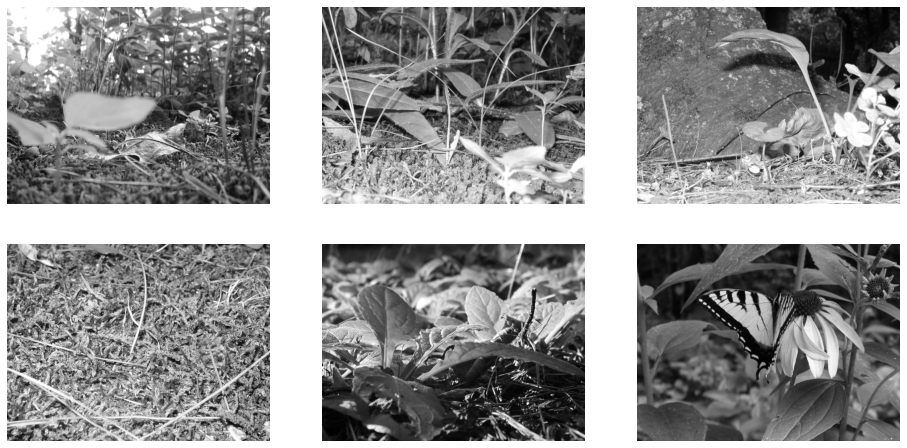
\includegraphics{./Natural Image Environment_files/figure-pdf/fig-orig-output-1.png}

}

\caption{\label{fig-orig}A Small Subset of the Original Natural Images}

\end{figure}

\begin{Shaded}
\begin{Highlighting}[]
\CommentTok{\# Make the logged image files}

\ControlFlowTok{if} \KeywordTok{not}\NormalTok{ os.path.exists(}\StringTok{\textquotesingle{}asdf/bbsk081604\_all\_log2dog.asdf\textquotesingle{}}\NormalTok{):}
\NormalTok{    im}\OperatorTok{=}\NormalTok{[np.log2(I}\OperatorTok{{-}}\NormalTok{I.}\BuiltInTok{min}\NormalTok{()}\OperatorTok{+}\DecValTok{1}\NormalTok{) }\ControlFlowTok{for}\NormalTok{ I }\KeywordTok{in}\NormalTok{ var[}\StringTok{\textquotesingle{}im\textquotesingle{}}\NormalTok{]]}
\NormalTok{    var\_log}\OperatorTok{=}\NormalTok{\{}\StringTok{\textquotesingle{}im\textquotesingle{}}\NormalTok{:im,}\StringTok{\textquotesingle{}im\_scale\_shift\textquotesingle{}}\NormalTok{:[}\FloatTok{1.0}\NormalTok{,}\FloatTok{0.0}\NormalTok{]\}}
\NormalTok{    var\_norm}\OperatorTok{=}\NormalTok{filters.make\_norm(var\_log)}
\NormalTok{    var\_dog}\OperatorTok{=}\NormalTok{filters.make\_dog(var\_norm)}
\NormalTok{    filters.set\_resolution(var\_dog,}\StringTok{\textquotesingle{}uint16\textquotesingle{}}\NormalTok{)}
\NormalTok{    pi5.asdf\_save\_images(var\_dog,}\StringTok{\textquotesingle{}asdf/bbsk081604\_all\_log2dog.asdf\textquotesingle{}}\NormalTok{) }
    \KeywordTok{del}\NormalTok{ var\_norm, var\_dog, var}
\end{Highlighting}
\end{Shaded}

\begin{Shaded}
\begin{Highlighting}[]
\NormalTok{fname}\OperatorTok{=}\StringTok{\textquotesingle{}asdf/bbsk081604\_all\_log2dog.asdf\textquotesingle{}}
\NormalTok{image\_data}\OperatorTok{=}\NormalTok{pi5.asdf\_load\_images(fname)}
\NormalTok{im}\OperatorTok{=}\NormalTok{[arr.astype(}\BuiltInTok{float}\NormalTok{)}\OperatorTok{*}\NormalTok{image\_data[}\StringTok{\textquotesingle{}im\_scale\_shift\textquotesingle{}}\NormalTok{][}\DecValTok{0}\NormalTok{]}\OperatorTok{+}
\NormalTok{        image\_data[}\StringTok{\textquotesingle{}im\_scale\_shift\textquotesingle{}}\NormalTok{][}\DecValTok{1}\NormalTok{] }\ControlFlowTok{for}\NormalTok{ arr }\KeywordTok{in}\NormalTok{ image\_data[}\StringTok{\textquotesingle{}im\textquotesingle{}}\NormalTok{]]}
\KeywordTok{del}\NormalTok{ image\_data}
\NormalTok{plt.figure(figsize}\OperatorTok{=}\NormalTok{(}\DecValTok{16}\NormalTok{,}\DecValTok{8}\NormalTok{))}
\ControlFlowTok{for}\NormalTok{ i }\KeywordTok{in} \BuiltInTok{range}\NormalTok{(}\DecValTok{6}\NormalTok{):}
\NormalTok{    plt.subplot(}\DecValTok{2}\NormalTok{,}\DecValTok{3}\NormalTok{,i}\OperatorTok{+}\DecValTok{1}\NormalTok{)}
\NormalTok{    plt.imshow(im[i],cmap}\OperatorTok{=}\NormalTok{plt.cm.gray)}
\NormalTok{    plt.axis(}\StringTok{\textquotesingle{}off\textquotesingle{}}\NormalTok{)}
\end{Highlighting}
\end{Shaded}

\begin{figure}[H]

{\centering 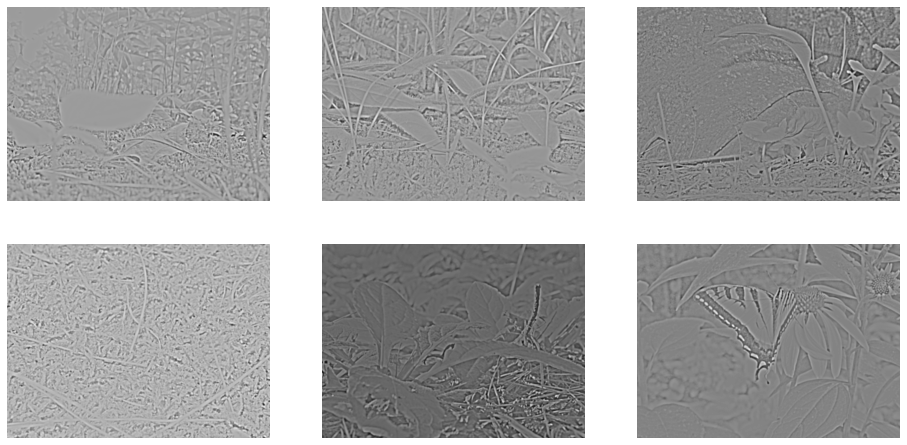
\includegraphics{./Natural Image Environment_files/figure-pdf/fig-logdog-output-1.png}

}

\caption{\label{fig-logdog}A Small Subset of the Natural Images filtered
with a base-2 Log function and a difference of Gaussians (DOG)}

\end{figure}

\hypertarget{two-eye-architecture}{%
\section{Two-eye architecture}\label{two-eye-architecture}}

Shown in Figure Figure~\ref{fig-arch} is the visual field, approximated
here as a two-dimensional projection, to left and right retinal cells.
These left and right retinal cells project to the left and right LGN
cells, respectively, and finally to a single cortical cell. The LGN is
assumed to be a simple relay, and does not modify the incoming retinal
activity. It is important to understand that the model we are pursuing
here is a \emph{single cortical cell} which receives input from both
eyes. We will encounter some limitations to this model which may
necessitate exploring multi-neuron systems.

In the model, normal development is simulated with identical image
patches presented to both eyes combined with small independent noise in
each eye. The random noise is generated from a zero-mean normal
distribution of a particular variance, representing the natural
variation in responses of LGN neurons. Practically, the independent
random noise added to each of the two-eye channels avoids the artificial
situation of having mathematically identical inputs in the channels. The
development of the deficit and the subsequent treatment protocols are
modeled with added preprocessing to these image patches, described later
in Chapter~\ref{sec-models-of-development} and
Chapter~\ref{sec-models-of-treatments}.

For all of the simulations we use a 19x19 receptive field, which is a
compromise between speed of simulation and the limits of spatial
discretization. We perform at least 20 independent simulations for each
condition to address variation in the results.

\begin{figure}

{\centering 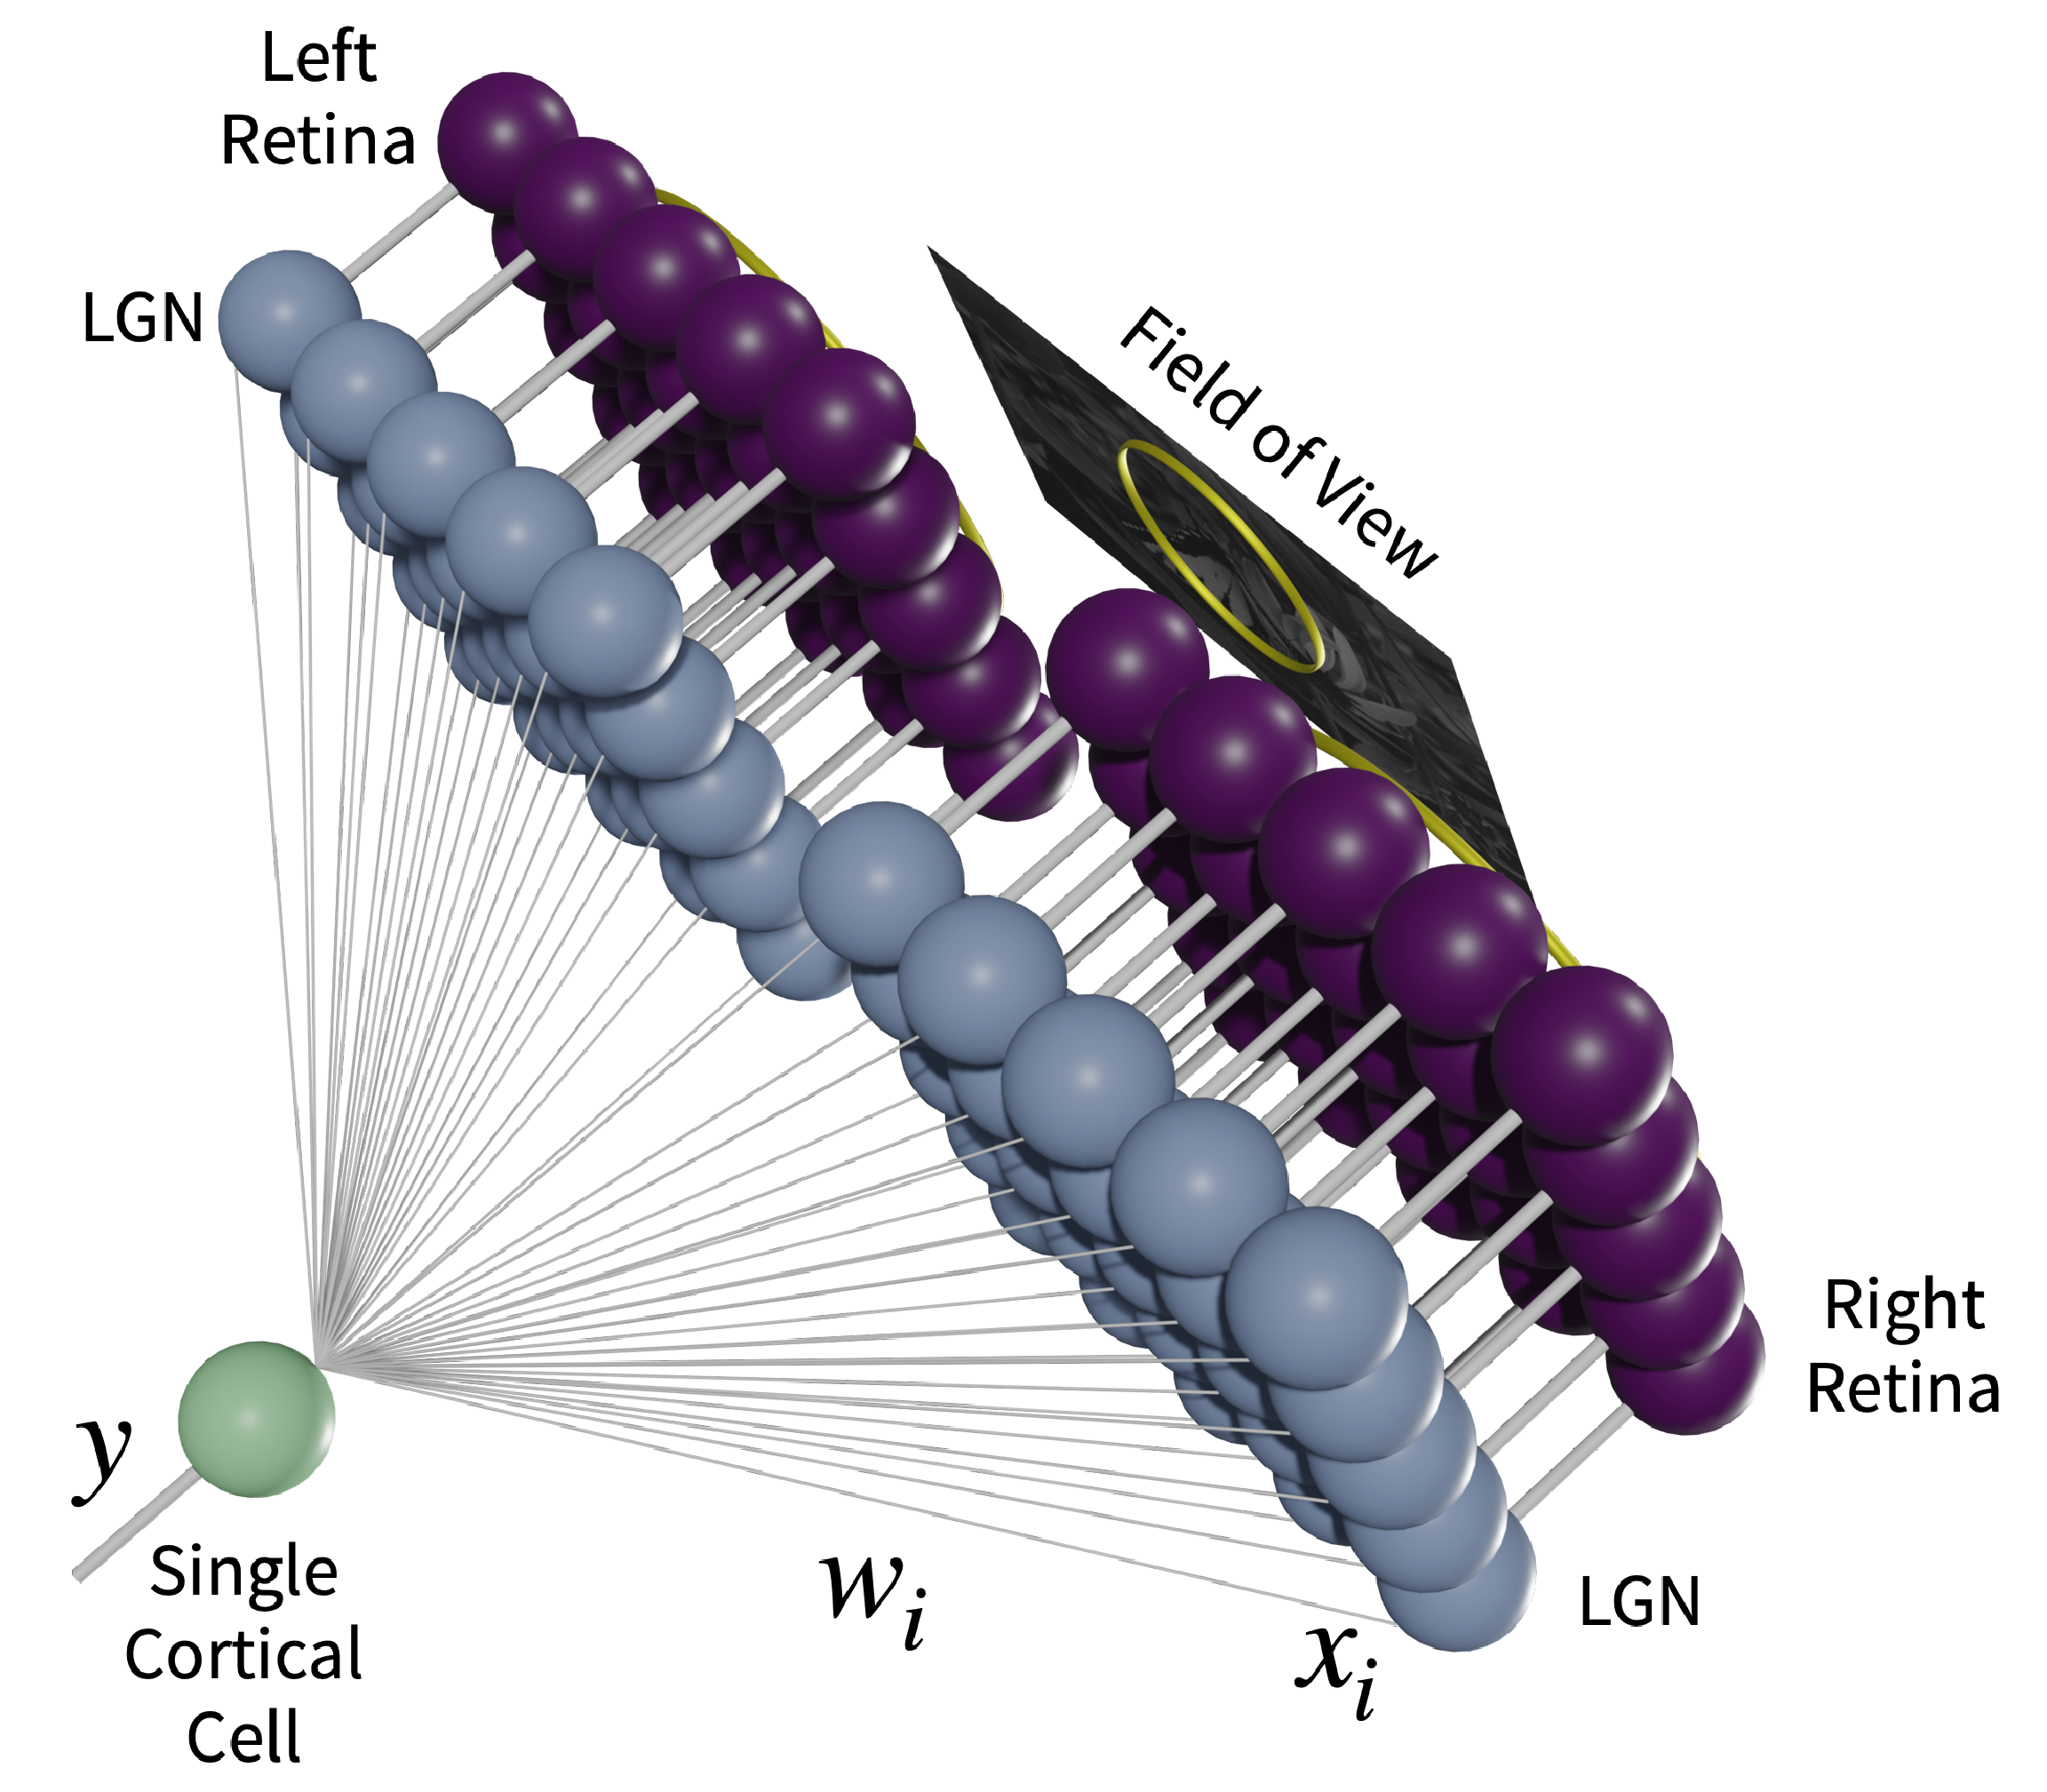
\includegraphics{./resources/arch.pdf}

}

\caption{\label{fig-arch}Two-eye Architecture.}

\end{figure}

\begin{Shaded}
\begin{Highlighting}[]
\NormalTok{sim,X}\OperatorTok{=}\NormalTok{get\_input\_patch\_examples(blur}\OperatorTok{={-}}\DecValTok{1}\NormalTok{)}
\NormalTok{ims}\OperatorTok{=}\NormalTok{inputs\_to\_images(X,}\BuiltInTok{buffer}\OperatorTok{=}\DecValTok{2}\NormalTok{)}
\NormalTok{figure(figsize}\OperatorTok{=}\NormalTok{(}\DecValTok{20}\NormalTok{,}\DecValTok{6}\NormalTok{))}
\ControlFlowTok{for}\NormalTok{ i }\KeywordTok{in} \BuiltInTok{range}\NormalTok{(}\DecValTok{24}\NormalTok{):}
\NormalTok{    im}\OperatorTok{=}\NormalTok{ims[i]}
\NormalTok{    subplot(}\DecValTok{4}\NormalTok{,}\DecValTok{6}\NormalTok{,i}\OperatorTok{+}\DecValTok{1}\NormalTok{)}
\NormalTok{    imshow(im,cmap}\OperatorTok{=}\NormalTok{plt.cm.gray)}
\NormalTok{    axis(}\StringTok{\textquotesingle{}off\textquotesingle{}}\NormalTok{)}
    
\end{Highlighting}
\end{Shaded}

\begin{figure}[H]

{\centering 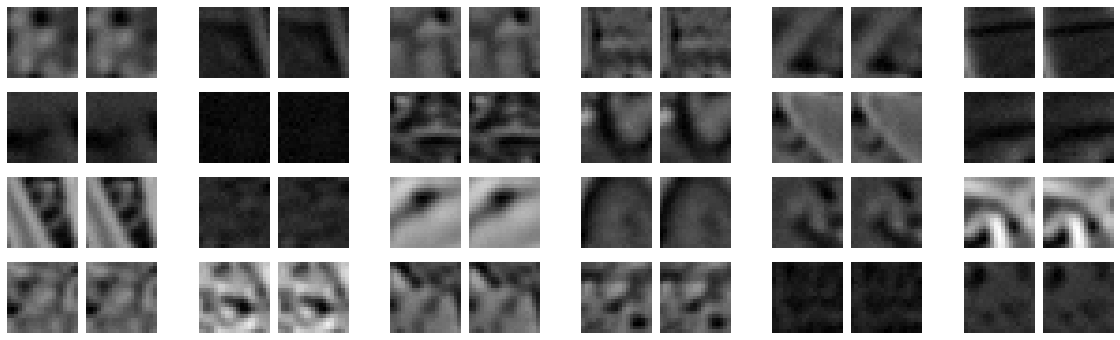
\includegraphics{./Natural Image Environment_files/figure-pdf/fig-normal-inputs-output-1.png}

}

\caption{\label{fig-normal-inputs}A sample of 24 input patches from a
normal visual environment. The left- and right-eye inputs are shown in
pairs.}

\end{figure}

\hypertarget{synaptic-modification}\NormalTok{matplotlib inline}
\ImportTok{from}\NormalTok{ input\_environment\_defs }\ImportTok{import} \OperatorTok{*}
\ImportTok{from}\NormalTok{ deficit\_defs }\ImportTok{import}\NormalTok{ Results}
\end{Highlighting}
\end{Shaded}

\hypertarget{the-bcm-learning-rule}{%
\section{The BCM Learning Rule}\label{the-bcm-learning-rule}}

We use a single neuron and the parabolic form of the BCM(Bienenstock,
Cooper, and Munro 1982; Brian S. Blais et al. 2008) learning rule for
all of the simulations, where the synaptic modification depends on the
postsynaptic activity, \(y\), in the following way for a single neuron

\[
y=\sigma\left(\sum_i x_i w_i \right)
\] \[
\frac{dw_i}{dt} = \eta y(y-\theta_M) x_i
\] \[
\frac{d\theta_M}{dt} = (y^2-\theta_M)/\tau
\]

where is \(x_i\) is the \(i\)th presynaptic input, \(w_i\) is the
\(i\)th synaptic weight, and \(y\) is the postsynaptic output activity.
The constant, \(\eta\), refers to the learning rate and the constant,
\(\tau\), is what we call the memory-constant and is related to the
speed of the sliding threshold. The transfer function,
\(\sigma(\cdot)\), places minimum and maximum responses given a set of
inputs and weights.

\begin{Shaded}
\begin{Highlighting}[]
\NormalTok{y}\OperatorTok{=}\NormalTok{np.linspace(}\OperatorTok{{-}}\DecValTok{5}\NormalTok{,}\DecValTok{20}\NormalTok{,}\DecValTok{100}\NormalTok{)}
\NormalTok{θ\_M}\OperatorTok{=}\DecValTok{8}
\NormalTok{ϕ}\OperatorTok{=}\NormalTok{y}\OperatorTok{*}\NormalTok{(y}\OperatorTok{{-}}\NormalTok{θ\_M)}

\NormalTok{plot(y,ϕ,}\StringTok{\textquotesingle{}b{-}\textquotesingle{}}\NormalTok{)}

\NormalTok{yl}\OperatorTok{=}\NormalTok{gca().get\_ylim()}
\NormalTok{plot([}\DecValTok{0}\NormalTok{,}\DecValTok{0}\NormalTok{],yl,}\StringTok{\textquotesingle{}k{-}{-}\textquotesingle{}}\NormalTok{)}
\NormalTok{gca().set\_ylim(yl)}

\NormalTok{xl}\OperatorTok{=}\NormalTok{gca().get\_xlim()}
\NormalTok{plot(xl,[}\DecValTok{0}\NormalTok{,}\DecValTok{0}\NormalTok{],}\StringTok{\textquotesingle{}k{-}{-}\textquotesingle{}}\NormalTok{)}
\NormalTok{gca().set\_xlim(xl)}

\NormalTok{plt.text(θ\_M,}\DecValTok{30}\NormalTok{,}\VerbatimStringTok{r\textquotesingle{}$\textbackslash{}theta\_M$\textquotesingle{}}\NormalTok{,ha}\OperatorTok{=}\StringTok{\textquotesingle{}center\textquotesingle{}}\NormalTok{,va}\OperatorTok{=}\StringTok{\textquotesingle{}center\textquotesingle{}}\NormalTok{)}
\NormalTok{plt.arrow(θ\_M}\OperatorTok{+}\DecValTok{1}\NormalTok{,}\DecValTok{30}\NormalTok{,}\DecValTok{5}\NormalTok{,}\DecValTok{0}\NormalTok{,color}\OperatorTok{=}\StringTok{\textquotesingle{}r\textquotesingle{}}\NormalTok{,length\_includes\_head}\OperatorTok{=}\VariableTok{True}\NormalTok{,}
\NormalTok{              head\_width}\OperatorTok{=}\DecValTok{5}\NormalTok{, head\_length}\OperatorTok{=}\FloatTok{.6}\NormalTok{,lw}\OperatorTok{=}\DecValTok{2}\NormalTok{)}
\NormalTok{plt.arrow(θ\_M}\OperatorTok{{-}}\DecValTok{1}\NormalTok{,}\DecValTok{30}\NormalTok{,}\OperatorTok{{-}}\DecValTok{5}\NormalTok{,}\DecValTok{0}\NormalTok{,color}\OperatorTok{=}\StringTok{\textquotesingle{}r\textquotesingle{}}\NormalTok{,length\_includes\_head}\OperatorTok{=}\VariableTok{True}\NormalTok{,}
\NormalTok{              head\_width}\OperatorTok{=}\DecValTok{5}\NormalTok{, head\_length}\OperatorTok{=}\FloatTok{.6}\NormalTok{,lw}\OperatorTok{=}\DecValTok{2}\NormalTok{)}
\NormalTok{plot([θ\_M,θ\_M],[}\OperatorTok{{-}}\DecValTok{10}\NormalTok{,}\DecValTok{10}\NormalTok{],}\StringTok{\textquotesingle{}r{-}\textquotesingle{}}\NormalTok{,lw}\OperatorTok{=}\DecValTok{2}\NormalTok{)}
\NormalTok{xlabel(}\StringTok{\textquotesingle{}Neuron output ($y$)\textquotesingle{}}\NormalTok{)}
\NormalTok{ylabel(}\StringTok{\textquotesingle{}Change in the synaptic weight ($dw/dt$)\textquotesingle{}}\NormalTok{)}\OperatorTok{;}
\end{Highlighting}
\end{Shaded}

\begin{figure}[H]

{\centering 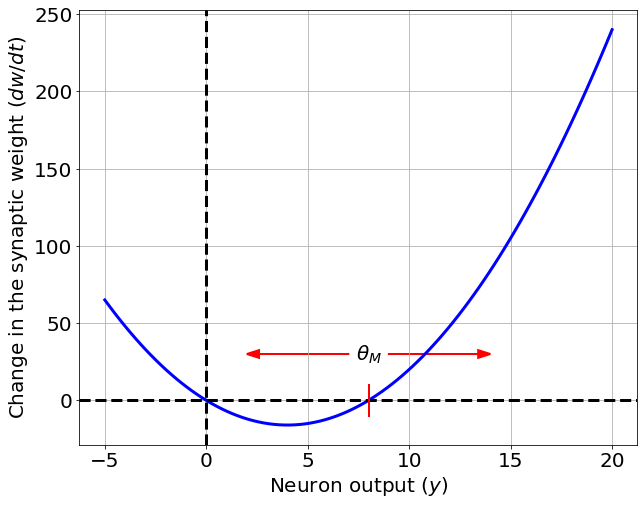
\includegraphics{./Synaptic Modification_files/figure-pdf/fig-phi-output-1.png}

}

\caption{\label{fig-phi}The BCM synaptic modification function. Units
are arbitrary.}

\end{figure}

The results are extremely robust to values of \(\eta\) and \(\tau\) ,
which are generally chosen for practical, rather than theoretical,
considerations. Each of these constants is related to the time-step for
the simulations, but given the phenomenological nature of the BCM theory
it is beyond the scope of this paper to make detailed comparisons
between simulation time and real-time. Further, the fact that \(\tau\)
can be changed within a factor of 100 with no noticeable effect, the
experiments presented here cannot be used address the time-scales of the
molecular mechanisms underlying synaptic modification. Whenever we refer
to real-time units for a simulation, we approximate a single simulation
iteration as 1 iteration = 0.2 seconds(Brian S. Blais 1998).

In the BCM learning rule, weights decrease if \(y\) is less than the
modification threshold,\(\theta_M\) , and increase if \(y\) is greater
than the modification threshold. To stabilize learning, the modification
threshold ``slides'' as a super-linear function of the output. The
output, \(y\) , is related to the product of the inputs and the weights
via a sigmoidal function, \(\sigma(\cdot)\), which places constraints on
the values of the output, keeping it in the range -1 and 50. The
interpretation of negative values is consistent with previous work(B. S.
Blais et al. 1998), where the activity values are measured relative to
spontaneous activity. Thus, negative values are interpreted as activity
below spontaneous. We continue this usage, in order to more easily
compare with previous simulations. The role of the spontaneous level for
the simulations in the natural image environment is discussed
elsewhere(B. S. Blais et al. 1998).

\hypertarget{simulation}{%
\section{Simulation}\label{simulation}}

The synaptic weights, and the modification threshold, are set to small
random initial values at the beginning of a simulation. At each
iteration, an input patch is generated as described above depending on
the procedure being simulated and then presented to the neuron. After
each input patch is presented, the weights are modified using the output
of the neuron, the input values and the current value of the
modification threshold. In an input environment composed of patches
taken from natural images, with equal patches presented to the left- and
right-eyes as shown in Figure~\ref{fig-normal-inputs}, this process
orientation selective and fully binocular cells(B. S. Blais et al.
1998). We then present test stimulus made from sine-gratings with 24
orientations, 20 spatial frequencies, and optimized over phase. Applying
any of the blur filters to the sine gratings does not quantitatively
change the result.

\begin{Shaded}
\begin{Highlighting}[]
\NormalTok{fname}\OperatorTok{=}\NormalTok{pi5.filtered\_images(}\StringTok{\textquotesingle{}asdf/bbsk081604\_all\_log2dog.asdf\textquotesingle{}}\NormalTok{)}

\NormalTok{pre1}\OperatorTok{=}\NormalTok{pn.neurons.natural\_images(fname,}
\NormalTok{                               rf\_size}\OperatorTok{=}\DecValTok{19}\NormalTok{,verbose}\OperatorTok{=}\VariableTok{False}\NormalTok{)}

\NormalTok{pre2}\OperatorTok{=}\NormalTok{pn.neurons.natural\_images(fname,rf\_size}\OperatorTok{=}\DecValTok{19}\NormalTok{,}
\NormalTok{                            other\_channel}\OperatorTok{=}\NormalTok{pre1,}
\NormalTok{                            verbose}\OperatorTok{=}\VariableTok{False}\NormalTok{)}

\NormalTok{pre1}\OperatorTok{+=}\NormalTok{pn.neurons.process.add\_noise\_normal(}\DecValTok{0}\NormalTok{,}\FloatTok{0.5}\NormalTok{) }\CommentTok{\# a little noise}
\NormalTok{pre2}\OperatorTok{+=}\NormalTok{pn.neurons.process.add\_noise\_normal(}\DecValTok{0}\NormalTok{,}\FloatTok{0.5}\NormalTok{) }\CommentTok{\# a little noise}


\NormalTok{pre}\OperatorTok{=}\NormalTok{pre1}\OperatorTok{+}\NormalTok{pre2}

\NormalTok{number\_of\_neurons}\OperatorTok{=}\DecValTok{5}
\NormalTok{post}\OperatorTok{=}\NormalTok{pn.neurons.linear\_neuron(number\_of\_neurons)}
\NormalTok{post}\OperatorTok{+=}\NormalTok{pn.neurons.process.sigmoid(}\DecValTok{0}\NormalTok{,}\DecValTok{50}\NormalTok{)}

\NormalTok{c}\OperatorTok{=}\NormalTok{pn.connections.BCM(pre,post,[}\OperatorTok{{-}}\FloatTok{.01}\NormalTok{,}\FloatTok{.01}\NormalTok{],[}\FloatTok{.1}\NormalTok{,}\FloatTok{.2}\NormalTok{])}
\NormalTok{c}\OperatorTok{+=}\NormalTok{pn.connections.process.orthogonalization(}\DecValTok{10}\OperatorTok{*}\NormalTok{minute)}
\NormalTok{c.eta}\OperatorTok{=}\FloatTok{2e{-}6}
\NormalTok{c.tau}\OperatorTok{=}\DecValTok{15}\OperatorTok{*}\NormalTok{minute   }

\NormalTok{sim}\OperatorTok{=}\NormalTok{pn.simulation(}\DecValTok{4}\OperatorTok{*}\NormalTok{day)}
\NormalTok{sim.dt}\OperatorTok{=}\DecValTok{200}\OperatorTok{*}\NormalTok{ms}

\NormalTok{save\_interval}\OperatorTok{=}\DecValTok{30}\OperatorTok{*}\NormalTok{minute}
\NormalTok{sim.monitor(post,[}\StringTok{\textquotesingle{}output\textquotesingle{}}\NormalTok{],save\_interval)}
\NormalTok{sim.monitor(c,[}\StringTok{\textquotesingle{}weights\textquotesingle{}}\NormalTok{,}\StringTok{\textquotesingle{}theta\textquotesingle{}}\NormalTok{],save\_interval)}

\NormalTok{sim}\OperatorTok{+=}\NormalTok{pn.grating\_response()}

\NormalTok{pn.run\_sim(sim,[pre,post],[c],display\_hash}\OperatorTok{=}\VariableTok{True}\NormalTok{,print\_time}\OperatorTok{=}\VariableTok{True}\NormalTok{)}
\NormalTok{pn.save(}\StringTok{\textquotesingle{}sims/nr.asdf\textquotesingle{}}\NormalTok{,sim,[pre,post],[c])}
\NormalTok{R}\OperatorTok{=}\NormalTok{Results(}\StringTok{\textquotesingle{}sims/nr.asdf\textquotesingle{}}\NormalTok{)}
\end{Highlighting}
\end{Shaded}

\begin{Shaded}
\begin{Highlighting}[]
\KeywordTok{def}\NormalTok{ argmax\_rc(X):}
    \CommentTok{"""Return the row and col of the maximum value"""}
\NormalTok{    r,c}\OperatorTok{=}\NormalTok{np.unravel\_index(np.argmax(X), X.shape)}
    \ControlFlowTok{return}\NormalTok{ r,c}
\end{Highlighting}
\end{Shaded}

\begin{Shaded}
\begin{Highlighting}[]
\NormalTok{figure(figsize}\OperatorTok{=}\NormalTok{(}\DecValTok{4}\NormalTok{,}\DecValTok{10}\NormalTok{))}
\NormalTok{R.plot\_rf()}

\NormalTok{figure(figsize}\OperatorTok{=}\NormalTok{(}\DecValTok{10}\NormalTok{,}\DecValTok{8}\NormalTok{))}
\NormalTok{plot(R.t}\OperatorTok{/}\NormalTok{hour,R.θ,label}\OperatorTok{=}\NormalTok{[}\SpecialStringTok{f\textquotesingle{}Neuron }\SpecialCharTok{\{}\NormalTok{i}\SpecialCharTok{\}}\SpecialStringTok{\textquotesingle{}} \ControlFlowTok{for}\NormalTok{ i }\KeywordTok{in}\NormalTok{ [}\DecValTok{0}\NormalTok{,}\DecValTok{1}\NormalTok{,}\DecValTok{2}\NormalTok{,}\DecValTok{3}\NormalTok{,}\DecValTok{4}\NormalTok{]])}
\NormalTok{ylabel(}\VerbatimStringTok{r\textquotesingle{}$\textbackslash{}theta\_M$\textquotesingle{}}\NormalTok{)}
\NormalTok{xlabel(}\StringTok{\textquotesingle{}Time (hours)\textquotesingle{}}\NormalTok{)}
\NormalTok{legend()}\OperatorTok{;}

\NormalTok{figure(figsize}\OperatorTok{=}\NormalTok{(}\DecValTok{10}\NormalTok{,}\DecValTok{8}\NormalTok{))}
\NormalTok{t,y}\OperatorTok{=}\NormalTok{R.all\_responses[}\DecValTok{0}\NormalTok{]}
\ControlFlowTok{for}\NormalTok{ neuron }\KeywordTok{in} \BuiltInTok{range}\NormalTok{(}\DecValTok{5}\NormalTok{):}
\NormalTok{    subplot(}\DecValTok{2}\NormalTok{,}\DecValTok{1}\NormalTok{,}\DecValTok{1}\NormalTok{)}
\NormalTok{    y\_left}\OperatorTok{=}\NormalTok{y[:,:,}\DecValTok{0}\NormalTok{,neuron,}\OperatorTok{{-}}\DecValTok{1}\NormalTok{]  }
\NormalTok{    y\_right}\OperatorTok{=}\NormalTok{y[:,:,}\DecValTok{1}\NormalTok{,neuron,}\OperatorTok{{-}}\DecValTok{1}\NormalTok{]  }
    
\NormalTok{    r,c}\OperatorTok{=}\NormalTok{argmax\_rc(y\_left)}
\NormalTok{    tuning\_curve}\OperatorTok{=}\NormalTok{y\_left[r,:]    }
\NormalTok{    plot(R.theta\_mat,tuning\_curve,}\StringTok{\textquotesingle{}{-}o\textquotesingle{}}\NormalTok{)}
\NormalTok{    plt.title(}\StringTok{\textquotesingle{}Left{-}eye Responses\textquotesingle{}}\NormalTok{)}
\NormalTok{    ylabel(}\StringTok{\textquotesingle{}Response\textquotesingle{}}\NormalTok{)}
\NormalTok{    gca().set\_xticklabels([])}
    
\NormalTok{    subplot(}\DecValTok{2}\NormalTok{,}\DecValTok{1}\NormalTok{,}\DecValTok{2}\NormalTok{)}
\NormalTok{    r,c}\OperatorTok{=}\NormalTok{argmax\_rc(y\_right)}
\NormalTok{    tuning\_curve}\OperatorTok{=}\NormalTok{y\_right[r,:]}
\NormalTok{    plot(R.theta\_mat,tuning\_curve,}\StringTok{\textquotesingle{}{-}s\textquotesingle{}}\NormalTok{)    }
\NormalTok{    plt.title(}\StringTok{\textquotesingle{}Right{-}eye Responses\textquotesingle{}}\NormalTok{)}
\NormalTok{    ylabel(}\StringTok{\textquotesingle{}Response\textquotesingle{}}\NormalTok{)}
\NormalTok{    xlabel(}\StringTok{\textquotesingle{}Angle of Stimulus\textquotesingle{}}\NormalTok{)}
    
\end{Highlighting}
\end{Shaded}

\begin{figure}

\begin{minipage}[t]{0.50\linewidth}

{\centering 

\raisebox{-\height}{

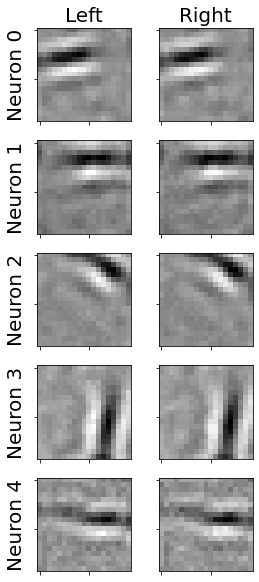
\includegraphics{./Synaptic Modification_files/figure-pdf/fig-nr_sim-output-1.png}

}

}

\subcaption{\label{fig-nr_sim-1}Synaptic weights where black denotes
weak weights and white denotes strone weights. A clear preference for
oriented stimuli can be seen.}
\end{minipage}%
%
\begin{minipage}[t]{0.50\linewidth}

{\centering 

\raisebox{-\height}{

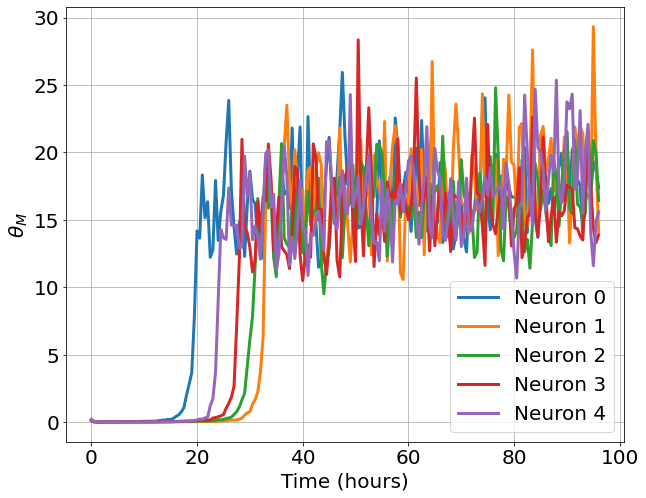
\includegraphics{./Synaptic Modification_files/figure-pdf/fig-nr_sim-output-2.png}

}

}

\subcaption{\label{fig-nr_sim-2}BCM modification threshold over time.
The value converges to nearly the same level for all neurons.}
\end{minipage}%
\newline
\begin{minipage}[t]{\linewidth}

{\centering 

\raisebox{-\height}{

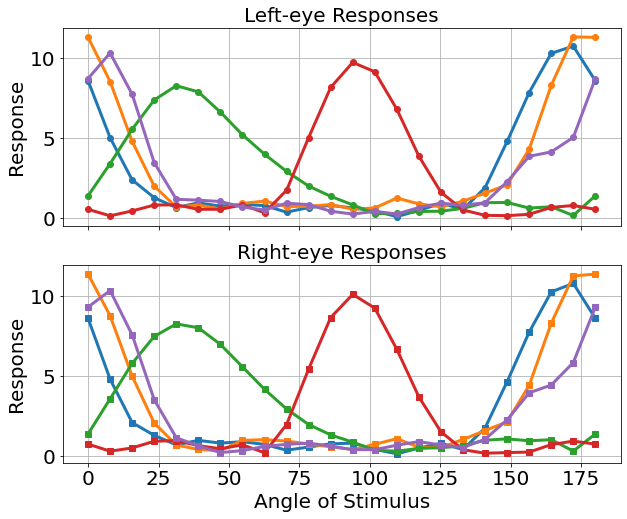
\includegraphics{./Synaptic Modification_files/figure-pdf/fig-nr_sim-output-3.png}

}

}

\subcaption{\label{fig-nr_sim-3}Responses to Oriented Stimuli after
training. Each neuron develops orientation selectivity to a range of
optimum angles.}
\end{minipage}%

\caption{\label{fig-nr_sim}Simulation of 5 neurons receiving identical
natural image patterns into the left- and right-input channels.}

\end{figure}

\hypertarget{sec-models-of-development}\NormalTok{matplotlib inline}
\ImportTok{from}\NormalTok{ input\_environment\_defs }\ImportTok{import} \OperatorTok{*}
\end{Highlighting}
\end{Shaded}

Amblyopia is a reduction of the best-corrected visual acuity (BCVA) with
an otherwise normal eye and has many causes(D. K. Wallace et al. 2018).
Two of the most common forms of amblyopia are strabismic and
anisometropic amblyiopia. Strabismic amblyopia occurs when the inputs
from each eye do not converge and the fixating eye becomes dominant over
a non-fixating eye. Refractive amblyopia occurs with untreated
unilateral refractive errors, one kind being anisometropic amblyopia
where unequal refractive power in each eye leads the retinal image from
the amblyopic eye to be blurred relative to the fellow eye. Both of
these processes lead to synaptic plasticity adjustments and interocular
competition, enhancing the initial deficit.

In this work we use a model of the amblyopic deficit caused by two
mechanisms. The first is a blurring of the amblyopic eye inputs,
representing refractive amblyopia. The second is eye-jitter,
representing one source of strabismic amblyopia. We can explore these
mechanisms independently and in conjunction to see how they respond
differentially to the various treatments.

\hypertarget{refractive-amblyopia}{%
\section{Refractive amblyopia}\label{refractive-amblyopia}}

The amblyopic eye is presented with image patches that have been
\emph{blurred} with a normalized Gaussian filter applied to the images
with a specified width. The larger the width the blurrier the resulting
filtered image.

\begin{Shaded}
\begin{Highlighting}[]
\NormalTok{sim,X}\OperatorTok{=}\NormalTok{get\_input\_patch\_examples(blur}\OperatorTok{=}\FloatTok{2.5}\NormalTok{)}
\NormalTok{ims}\OperatorTok{=}\NormalTok{inputs\_to\_images(X,}\BuiltInTok{buffer}\OperatorTok{=}\DecValTok{2}\NormalTok{)}
\NormalTok{figure(figsize}\OperatorTok{=}\NormalTok{(}\DecValTok{20}\NormalTok{,}\DecValTok{6}\NormalTok{))}
\ControlFlowTok{for}\NormalTok{ i }\KeywordTok{in} \BuiltInTok{range}\NormalTok{(}\DecValTok{24}\NormalTok{):}
\NormalTok{    im}\OperatorTok{=}\NormalTok{ims[i]}
\NormalTok{    subplot(}\DecValTok{4}\NormalTok{,}\DecValTok{6}\NormalTok{,i}\OperatorTok{+}\DecValTok{1}\NormalTok{)}
\NormalTok{    imshow(im,cmap}\OperatorTok{=}\NormalTok{plt.cm.gray)}
\NormalTok{    axis(}\StringTok{\textquotesingle{}off\textquotesingle{}}\NormalTok{)}
    
\end{Highlighting}
\end{Shaded}

\begin{figure}[H]

{\centering 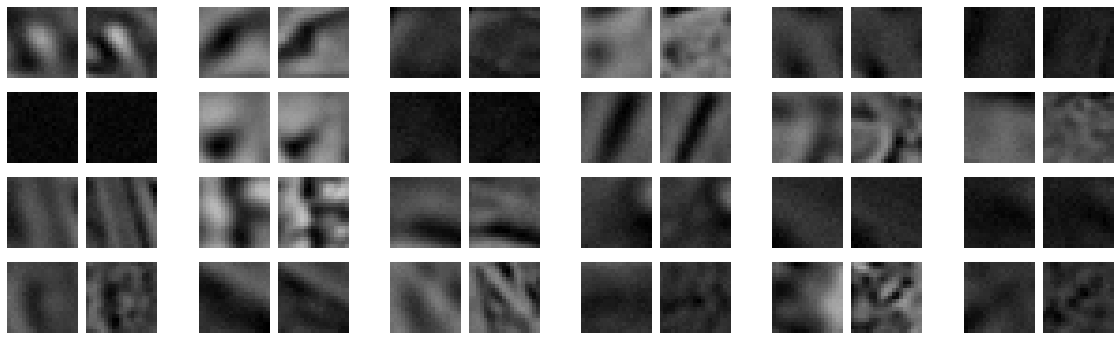
\includegraphics{./Deficit Models_files/figure-pdf/fig-blurred-inputs-output-1.png}

}

\caption{\label{fig-blurred-inputs}A sample of 24 input patches from a
refractive amblyopic environment. The amblyopic (blurred) input is the
square on the left-hand side of each pair.}

\end{figure}

\hypertarget{strabismic-amblyopia}{%
\section{Strabismic amblyopia}\label{strabismic-amblyopia}}

Strabismic inputs are modeled by changing the center of the left- and
right-input patches in a systematic way, with a set mean offset and a
standard deviation per input patch generated. In this way we can model
completely overlapping (i.e.~normal) inputs, completely non-overlapping
(i.e.~extreme strabismus), and any amount of overlap in between. Some
examples are shown in Figure~\ref{fig-jitter-inputs} with the offset
locations shown in Figure~\ref{fig-jitter-input-locations}.

\begin{Shaded}
\begin{Highlighting}[]
\NormalTok{mu\_r,mu\_c}\OperatorTok{=}\DecValTok{2}\NormalTok{,}\DecValTok{10}
\NormalTok{sigma\_r,sigma\_c}\OperatorTok{=}\DecValTok{1}\NormalTok{,}\DecValTok{2}

\NormalTok{sim,X}\OperatorTok{=}\NormalTok{get\_input\_patch\_examples\_with\_jitter(blur}\OperatorTok{={-}}\DecValTok{1}\NormalTok{,mu\_r}\OperatorTok{=}\NormalTok{mu\_r,mu\_c}\OperatorTok{=}\NormalTok{mu\_c,sigma\_r}\OperatorTok{=}\NormalTok{sigma\_r,sigma\_c}\OperatorTok{=}\NormalTok{sigma\_c)}
\NormalTok{ims}\OperatorTok{=}\NormalTok{inputs\_to\_images(X,}\BuiltInTok{buffer}\OperatorTok{=}\DecValTok{2}\NormalTok{)}
\NormalTok{figure(figsize}\OperatorTok{=}\NormalTok{(}\DecValTok{20}\NormalTok{,}\DecValTok{6}\NormalTok{))}
\ControlFlowTok{for}\NormalTok{ i }\KeywordTok{in} \BuiltInTok{range}\NormalTok{(}\DecValTok{24}\NormalTok{):}
\NormalTok{    im}\OperatorTok{=}\NormalTok{ims[i]}
\NormalTok{    subplot(}\DecValTok{4}\NormalTok{,}\DecValTok{6}\NormalTok{,i}\OperatorTok{+}\DecValTok{1}\NormalTok{)}
\NormalTok{    imshow(im,cmap}\OperatorTok{=}\NormalTok{plt.cm.gray)}
\NormalTok{    axis(}\StringTok{\textquotesingle{}off\textquotesingle{}}\NormalTok{)}
    
\end{Highlighting}
\end{Shaded}

\begin{figure}[H]

{\centering 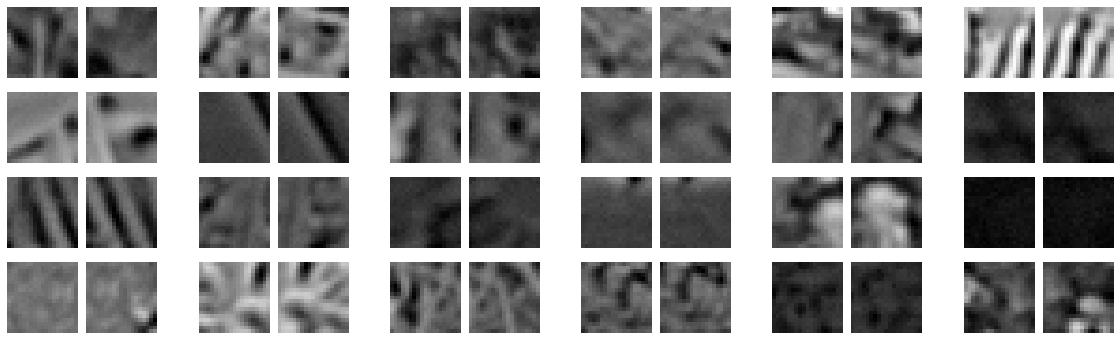
\includegraphics{./Deficit Models_files/figure-pdf/fig-jitter-inputs-output-1.png}

}

\caption{\label{fig-jitter-inputs}A sample of 24 input patches from a
strabismic visual environment achieved through random jitter of the
amblyopic (left) eye.}

\end{figure}

\begin{Shaded}
\begin{Highlighting}[]
\ImportTok{import}\NormalTok{ matplotlib.patches }\ImportTok{as}\NormalTok{ patches}
\NormalTok{ca}\OperatorTok{=}\NormalTok{sim.monitors[}\StringTok{\textquotesingle{}ca\textquotesingle{}}\NormalTok{].array()}
\NormalTok{ra}\OperatorTok{=}\NormalTok{sim.monitors[}\StringTok{\textquotesingle{}ra\textquotesingle{}}\NormalTok{].array()}
\NormalTok{c}\OperatorTok{=}\NormalTok{sim.monitors[}\StringTok{\textquotesingle{}c\textquotesingle{}}\NormalTok{].array()}
\NormalTok{r}\OperatorTok{=}\NormalTok{sim.monitors[}\StringTok{\textquotesingle{}r\textquotesingle{}}\NormalTok{].array()}

\NormalTok{ca\_1}\OperatorTok{=}\NormalTok{sim.monitors[}\StringTok{\textquotesingle{}ca\_1\textquotesingle{}}\NormalTok{].array()}
\NormalTok{ra\_1}\OperatorTok{=}\NormalTok{sim.monitors[}\StringTok{\textquotesingle{}ra\_1\textquotesingle{}}\NormalTok{].array()}
\NormalTok{c\_1}\OperatorTok{=}\NormalTok{sim.monitors[}\StringTok{\textquotesingle{}c\_1\textquotesingle{}}\NormalTok{].array()}
\NormalTok{r\_1}\OperatorTok{=}\NormalTok{sim.monitors[}\StringTok{\textquotesingle{}r\_1\textquotesingle{}}\NormalTok{].array()}

\NormalTok{figure(figsize}\OperatorTok{=}\NormalTok{(}\DecValTok{11}\NormalTok{,}\DecValTok{9}\NormalTok{))}
\NormalTok{plot(ca}\OperatorTok{{-}}\NormalTok{c,}\OperatorTok{{-}}\NormalTok{(ra}\OperatorTok{{-}}\NormalTok{r),}\StringTok{\textquotesingle{}bo\textquotesingle{}}\NormalTok{,label}\OperatorTok{=}\StringTok{\textquotesingle{}Left\textquotesingle{}}\NormalTok{)}

\NormalTok{plot(ca\_1}\OperatorTok{{-}}\NormalTok{c\_1,}\OperatorTok{{-}}\NormalTok{(ra\_1}\OperatorTok{{-}}\NormalTok{r\_1),}\StringTok{\textquotesingle{}ro\textquotesingle{}}\NormalTok{,label}\OperatorTok{=}\StringTok{\textquotesingle{}Right\textquotesingle{}}\NormalTok{)}
\NormalTok{rect }\OperatorTok{=}\NormalTok{ patches.Rectangle((}\OperatorTok{{-}}\DecValTok{19}\OperatorTok{/}\DecValTok{2}\NormalTok{, }\OperatorTok{{-}}\DecValTok{19}\OperatorTok{/}\DecValTok{2}\NormalTok{), }\DecValTok{19}\NormalTok{, }\DecValTok{19}\NormalTok{, linewidth}\OperatorTok{=}\DecValTok{1}\NormalTok{, edgecolor}\OperatorTok{=}\StringTok{\textquotesingle{}b\textquotesingle{}}\NormalTok{,lw}\OperatorTok{=}\DecValTok{2}\NormalTok{, facecolor}\OperatorTok{=}\StringTok{\textquotesingle{}gray\textquotesingle{}}\NormalTok{,alpha}\OperatorTok{=}\FloatTok{0.5}\NormalTok{)}
\NormalTok{gca().add\_patch(rect)}
\NormalTok{rect }\OperatorTok{=}\NormalTok{ patches.Rectangle((}\OperatorTok{{-}}\DecValTok{19}\OperatorTok{/}\DecValTok{2}\OperatorTok{+}\NormalTok{mu\_c, }\OperatorTok{{-}}\DecValTok{19}\OperatorTok{/}\DecValTok{2}\OperatorTok{{-}}\NormalTok{mu\_r), }\DecValTok{19}\NormalTok{, }\DecValTok{19}\NormalTok{, linewidth}\OperatorTok{=}\DecValTok{1}\NormalTok{, edgecolor}\OperatorTok{=}\StringTok{\textquotesingle{}r\textquotesingle{}}\NormalTok{, lw}\OperatorTok{=}\DecValTok{2}\NormalTok{,facecolor}\OperatorTok{=}\StringTok{\textquotesingle{}gray\textquotesingle{}}\NormalTok{,alpha}\OperatorTok{=}\FloatTok{0.5}\NormalTok{)}
\NormalTok{gca().add\_patch(rect)}
\NormalTok{axis(}\StringTok{\textquotesingle{}equal\textquotesingle{}}\NormalTok{)}\OperatorTok{;}

\NormalTok{xlabel(}\StringTok{\textquotesingle{}Horizontal Visual Field Location (pixels)\textquotesingle{}}\NormalTok{)}
\NormalTok{ylabel(}\StringTok{\textquotesingle{}Vertical Visual Field Location (pixels)\textquotesingle{}}\NormalTok{)}\OperatorTok{;}
\NormalTok{legend()}\OperatorTok{;}
\end{Highlighting}
\end{Shaded}

\begin{figure}[H]

{\centering 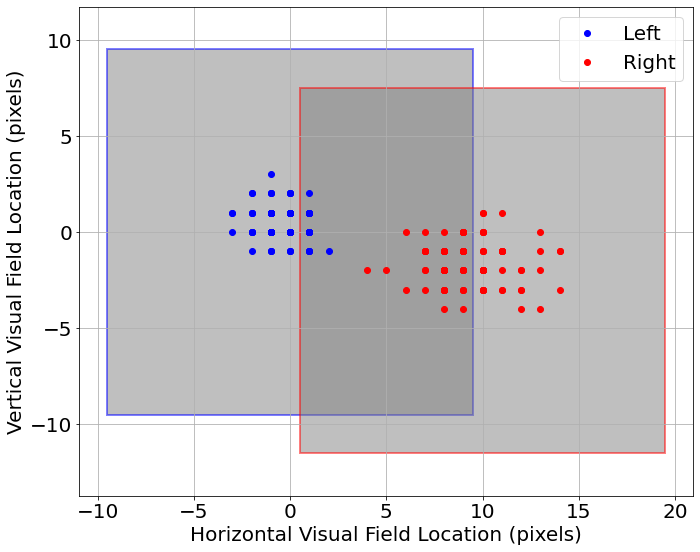
\includegraphics{./Deficit Models_files/figure-pdf/fig-jitter-input-locations-output-1.png}

}

\caption{\label{fig-jitter-input-locations}Locations of the center of
the left- and right-field of view receptive fields, jittered randomly
with set mean and standard deviation. The average receptive fields are
shown as gray squares.}

\end{figure}

\hypertarget{sec-models-of-treatments}\NormalTok{matplotlib inline}
\ImportTok{import}\NormalTok{ matplotlib.pyplot }\ImportTok{as}\NormalTok{ plt}
\ImportTok{import}\NormalTok{ numpy }\ImportTok{as}\NormalTok{ np}
\ImportTok{import}\NormalTok{ plasticnet }\ImportTok{as}\NormalTok{ pn}
\ImportTok{import}\NormalTok{ process\_images\_hdf5 }\ImportTok{as}\NormalTok{ pi5}
\ImportTok{from}\NormalTok{ deficit\_defs }\ImportTok{import}\NormalTok{ patch\_treatment}
\ImportTok{from}\NormalTok{ input\_environment\_defs }\ImportTok{import}\NormalTok{ get\_input\_patch\_examples}
\ImportTok{from}\NormalTok{ matplotlib.pyplot }\ImportTok{import}\NormalTok{ figure,xlabel,ylabel,legend,gca,plot,subplot,imshow,axis}
\end{Highlighting}
\end{Shaded}

To model the fix to the refractive imbalance we follow the deficit
simulation with an input environment that is rebalanced, both eyes
receiving nearly identical input patches
(Figure~\ref{fig-normal-inputs}). This process is a model of the
application of refractive correction. Although both eyes receive nearly
identical input patches, we add independent Gaussian noise to each input
channel to represent the natural variation in the activity in each eye.
In addition, in those cases where use employ strabismic amblyopia, the
inter-eye jitter is not corrected with the refractive correction.

\begin{Shaded}
\begin{Highlighting}[]
\KeywordTok{def}\NormalTok{ inputs\_to\_images1(X,}\BuiltInTok{buffer}\OperatorTok{=}\DecValTok{5}\NormalTok{):}
\NormalTok{    ims}\OperatorTok{=}\NormalTok{[]}
    
\NormalTok{    rf\_size}\OperatorTok{=}\BuiltInTok{int}\NormalTok{(np.sqrt(X.shape[}\DecValTok{1}\NormalTok{]}\OperatorTok{/}\DecValTok{2}\NormalTok{))}
\NormalTok{    vmax}\OperatorTok{=}\NormalTok{np.concatenate([xx[:rf\_size}\OperatorTok{*}\NormalTok{rf\_size] }\ControlFlowTok{for}\NormalTok{ xx }\KeywordTok{in}\NormalTok{ X]).}\BuiltInTok{max}\NormalTok{()}
    
    \ControlFlowTok{for}\NormalTok{ xx }\KeywordTok{in}\NormalTok{ X:}
\NormalTok{        xx1}\OperatorTok{=}\NormalTok{xx[:rf\_size}\OperatorTok{*}\NormalTok{rf\_size].reshape(rf\_size,rf\_size)}
\NormalTok{        im}\OperatorTok{=}\NormalTok{xx1}
\NormalTok{        ims.append(im)}
        
    \ControlFlowTok{return}\NormalTok{ ims}

\KeywordTok{def}\NormalTok{ inputs\_to\_images2(X,}\BuiltInTok{buffer}\OperatorTok{=}\DecValTok{5}\NormalTok{):}
\NormalTok{    ims}\OperatorTok{=}\NormalTok{[]}
    
\NormalTok{    rf\_size}\OperatorTok{=}\BuiltInTok{int}\NormalTok{(np.sqrt(X.shape[}\DecValTok{1}\NormalTok{]}\OperatorTok{/}\DecValTok{2}\NormalTok{))}
\NormalTok{    vmax}\OperatorTok{=}\NormalTok{np.concatenate([xx[rf\_size}\OperatorTok{*}\NormalTok{rf\_size:] }\ControlFlowTok{for}\NormalTok{ xx }\KeywordTok{in}\NormalTok{ X]).}\BuiltInTok{max}\NormalTok{()}
    
    \ControlFlowTok{for}\NormalTok{ xx }\KeywordTok{in}\NormalTok{ X:}
\NormalTok{        xx2}\OperatorTok{=}\NormalTok{xx[rf\_size}\OperatorTok{*}\NormalTok{rf\_size:].reshape(rf\_size,rf\_size)}
\NormalTok{        im}\OperatorTok{=}\NormalTok{xx2}
\NormalTok{        ims.append(im)}
        
    \ControlFlowTok{return}\NormalTok{ ims}

\KeywordTok{def}\NormalTok{ inputs\_to\_images(X,}\BuiltInTok{buffer}\OperatorTok{=}\DecValTok{5}\NormalTok{):}
\NormalTok{    ims}\OperatorTok{=}\NormalTok{[]}
\NormalTok{    vmin}\OperatorTok{=}\NormalTok{X.}\BuiltInTok{min}\NormalTok{()}
\NormalTok{    vmax}\OperatorTok{=}\NormalTok{X.}\BuiltInTok{max}\NormalTok{()}
    
\NormalTok{    rf\_size}\OperatorTok{=}\BuiltInTok{int}\NormalTok{(np.sqrt(X.shape[}\DecValTok{1}\NormalTok{]}\OperatorTok{/}\DecValTok{2}\NormalTok{))}
        
    \ControlFlowTok{for}\NormalTok{ xx }\KeywordTok{in}\NormalTok{ X:}
\NormalTok{        xx1}\OperatorTok{=}\NormalTok{xx[:rf\_size}\OperatorTok{*}\NormalTok{rf\_size].reshape(rf\_size,rf\_size)}
\NormalTok{        xx2}\OperatorTok{=}\NormalTok{xx[rf\_size}\OperatorTok{*}\NormalTok{rf\_size:].reshape(rf\_size,rf\_size)}
\NormalTok{        im}\OperatorTok{=}\NormalTok{np.concatenate((xx1,np.ones((rf\_size,}\BuiltInTok{buffer}\NormalTok{))}\OperatorTok{*}\NormalTok{vmax,xx2),axis}\OperatorTok{=}\DecValTok{1}\NormalTok{)   }
\NormalTok{        ims.append(im)}
        
    \ControlFlowTok{return}\NormalTok{ ims}

\KeywordTok{def}\NormalTok{ get\_input\_patch\_examples\_treatment():}
    
\NormalTok{    seq}\OperatorTok{=}\NormalTok{pn.Sequence()    }
\NormalTok{    seq}\OperatorTok{+=}\NormalTok{patch\_treatment(patch\_noise}\OperatorTok{=}\FloatTok{0.5}\NormalTok{,}
\NormalTok{               total\_time}\OperatorTok{=}\DecValTok{1000}\NormalTok{,number\_of\_neurons}\OperatorTok{=}\DecValTok{1}\NormalTok{,}
\NormalTok{               eta}\OperatorTok{=}\FloatTok{1e{-}6}\NormalTok{,}
\NormalTok{               save\_interval}\OperatorTok{=}\DecValTok{1}\NormalTok{)}
\NormalTok{    sim}\OperatorTok{=}\NormalTok{seq.sims[}\DecValTok{0}\NormalTok{]}
\NormalTok{    pre}\OperatorTok{=}\NormalTok{seq[}\DecValTok{0}\NormalTok{][}\DecValTok{1}\NormalTok{][}\DecValTok{0}\NormalTok{]}
\NormalTok{    sim.monitor(pre,[}\StringTok{\textquotesingle{}output\textquotesingle{}}\NormalTok{],}\DecValTok{1}\NormalTok{)}

\NormalTok{    seq.run(display\_hash}\OperatorTok{=}\VariableTok{False}\NormalTok{,print\_time}\OperatorTok{=}\VariableTok{False}\NormalTok{)}
\NormalTok{    m}\OperatorTok{=}\NormalTok{sim.monitors[}\StringTok{\textquotesingle{}output\_1\textquotesingle{}}\NormalTok{]}
\NormalTok{    t,X}\OperatorTok{=}\NormalTok{m.arrays()    }
    
    \ControlFlowTok{return}\NormalTok{ seq,X}
\end{Highlighting}
\end{Shaded}

\hypertarget{patch-treatment}{%
\section{Patch treatment}\label{patch-treatment}}

The typical patch treatment is done by depriving the strong-eye of input
with an eye-patch. In the model this is equivalent to presenting the
strong-eye with random noise instead of the natural image input.
Competition between the left- and right-channels drives the recovery,
and is produced from the difference between \emph{structured} input into
the weak-eye and the \emph{unstructured} (i.e.~noise) input into the
strong eye. It is not driven by a reduction in input activity.
Figure~\ref{fig-patch-inputs} shows sample simulation input patterns
from the patched eye. Compare this to Figure~\ref{fig-normal-inputs} to
see that the simulated patch has far less structure than the normal
inputs.

\begin{figure}

{\centering 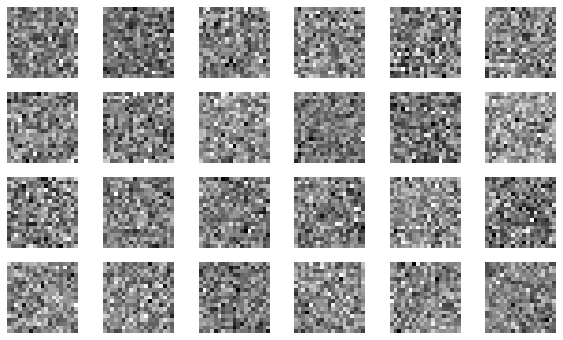
\includegraphics{./Treatment Models_files/figure-pdf/fig-patch-inputs-output-1.png}

}

\caption{\label{fig-patch-inputs}A sample of 24 input patches from a
patched visual environment.}

\end{figure}

\hypertarget{contrast-modification}{%
\section{Contrast modification}\label{contrast-modification}}

A binocular approach to treatment can be produced with contrast
reduction of the non-deprived channel relative to the deprived channel.
Experimentally this can be accomplished with VR headsets(Xiao et al.
2020). In the model we implement this by down-scaling the normal,
unblurred channel with a simple scalar multiplier applied to each pixel
(Figure \protect\hyperlink{fig:input}{4} D). The contrast difference
sets up competition between the two channels with the advantage given to
the weak-eye channel.

\begin{Shaded}
\begin{Highlighting}[]
\NormalTok{sim,X}\OperatorTok{=}\NormalTok{get\_input\_patch\_examples(blur}\OperatorTok{={-}}\DecValTok{1}\NormalTok{,contrast}\OperatorTok{=}\FloatTok{0.3}\NormalTok{)}
\NormalTok{ims}\OperatorTok{=}\NormalTok{inputs\_to\_images(X,}\BuiltInTok{buffer}\OperatorTok{=}\DecValTok{2}\NormalTok{)}
\NormalTok{figure(figsize}\OperatorTok{=}\NormalTok{(}\DecValTok{20}\NormalTok{,}\DecValTok{6}\NormalTok{))}
\ControlFlowTok{for}\NormalTok{ i }\KeywordTok{in} \BuiltInTok{range}\NormalTok{(}\DecValTok{24}\NormalTok{):}
\NormalTok{    im}\OperatorTok{=}\NormalTok{ims[i]}
\NormalTok{    subplot(}\DecValTok{4}\NormalTok{,}\DecValTok{6}\NormalTok{,i}\OperatorTok{+}\DecValTok{1}\NormalTok{)}
\NormalTok{    imshow(im,cmap}\OperatorTok{=}\NormalTok{plt.cm.gray)}
\NormalTok{    axis(}\StringTok{\textquotesingle{}off\textquotesingle{}}\NormalTok{)}
    
\end{Highlighting}
\end{Shaded}

\begin{figure}[H]

{\centering 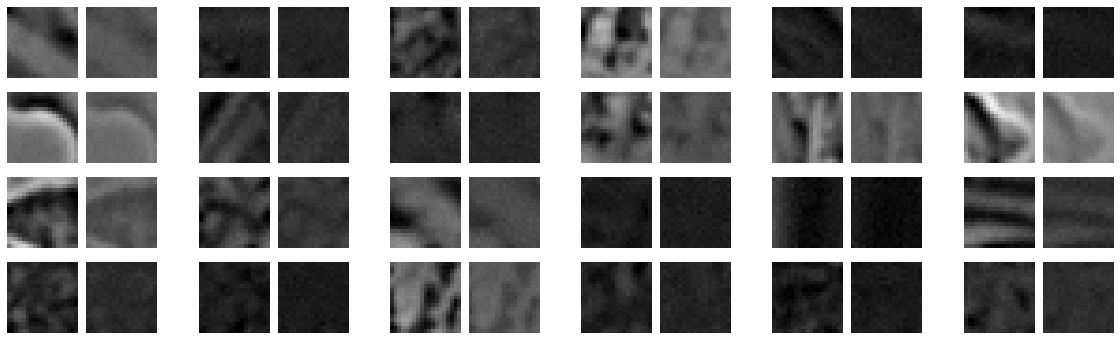
\includegraphics{./Treatment Models_files/figure-pdf/fig-contrast-modified-inputs-output-1.png}

}

\caption{\label{fig-contrast-modified-inputs}A sample of 24 input
patches from a normal visual environment with the right-channel
down-scaled relative to the left.}

\end{figure}

\hypertarget{dichoptic-mask}{%
\section{Dichoptic Mask}\label{dichoptic-mask}}

On top of the contrast modification, we can include the application of
the dichoptic mask (Figure (\textbf{fig:input?}) E). In this method,
each eye receives a version of the input images filtered through
independent masks in each channel, resulting in a mostly-independent
pattern in each channel.\\
It has been observed that contrast modification combined with dichoptic
masks can be an effective treatment for
amblyopia(\textbf{xiao2021randomized?}). The motivation behind the
application of the mask filter is that the neural system must use both
channels to reconstruct the full image and thus may lead to enhanced
recovery.

The dichoptic masks are constructed with the following procedure. A
blank image (i.e.~all zeros) is made to which is added 15 randomly sized
circles with values equal to 1 (Figure (\textbf{fig:dichopic\_blob?})).
These images are then smoothed with a Gaussian filter of a given width,
\(f\). This width is a parameter we can vary to change the overlap
between the left- and right-eye images. A high value of \(f\) compared
with the size of the receptive field, e.g.~\(f=90\), yields a high
overlap between the patterns in the weak- and strong-eye inputs (Figure
(\textbf{fig:dichopic\_filter\_size?})). Likewise, a small value of
\(f\), e.g.~\(f=10\), the eye inputs are nearly independent -- the
patterned activity falling mostly on one of the eyes and not much to
both. Finally, the smoothed images are scaled to have values from a
minimum of 0 to a maximum of 1. This image-mask we will call \(A\), and
is the left-eye mask whereas the right-eye mask, \(F\), is the inverse
of the left-eye mask, \(F\equiv 1-A\). The mask is applied to an image
by multiplying the left- and right-eye images by the left- and right-eye
masks, respectively, resulting in a pair of images which have no overlap
at the peaks of each mask, and nearly equal overlap in the areas of the
images where the masks are near 0.5 (Figure
(\textbf{fig:dichopic\_filter\_image?})).

\hypertarget{atropine-treatment}{%
\section{Atropine treatment}\label{atropine-treatment}}

In the atropine treatment for amblyopia(Glaser et al. 2002), eye-drops
of atropine are applied to the strong-eye resulting in blurred vision in
that eye. Here we use the same blurred filter used to obtain the deficit
(possibly with a different width) applied to the strong eye (Figure
(\textbf{fig:input?}) F). The difference in sharpness between the
strong-eye inputs and the weak-eye inputs sets up competition between
the two channels with the advantage given to the weak-eye.

\hypertarget{ocular-dominance-index}{%
\chapter{Ocular Dominance Index}\label{ocular-dominance-index}}

Simulations are ended when selectivity has been achieved and the
responses are stable. From the maximal responses of each eye,
\(R_{\text{left}}\) and \(R_{\text{right}}\), individually, we can
calculate the ocular dominance index as \[
\text{ODI} \equiv \frac{R_{\text{right}}-R_{\text{left}}}{R_{\text{right}}+R_{\text{left}}}
\] The ocular dominance index (ODI) has a value of
\(\text{ODI} \approx 1\) when stimulus to the right-eye (typically the
strong eye in the simulations, by convention) yields a maximum neuronal
response with little or no contribution from the left-eye. Likewise, an
ocular dominance index (ODI) has a value of \(\text{ODI} \approx -1\)
when stimulus to the left-eye (typically the weak eye, by convention)
yields a maximum neuronal response with little or no contribution from
the right-eye. A value of \(\text{ODI} \approx 0\) represents a purely
binocular cell, responding equally to stimulus in either eye.

\begin{tcolorbox}[enhanced jigsaw, toprule=.15mm, bottomrule=.15mm, colframe=quarto-callout-important-color-frame, colbacktitle=quarto-callout-important-color!10!white, breakable, bottomtitle=1mm, opacitybacktitle=0.6, colback=white, toptitle=1mm, arc=.35mm, title=\textcolor{quarto-callout-important-color}{\faExclamation}\hspace{0.5em}{Important}, opacityback=0, titlerule=0mm, rightrule=.15mm, left=2mm, leftrule=.75mm, coltitle=black]

\begin{itemize}
\tightlist
\item
  do an orientation tuning index
\item
  do a spatial frequency tuning index
\end{itemize}

\end{tcolorbox}

\part{Results}

\hypertarget{deficit-and-measuring-the-effectiveness-of-a-treatment}{%
\chapter{Deficit and Measuring the Effectiveness of a
Treatment}\label{deficit-and-measuring-the-effectiveness-of-a-treatment}}

Figure (\textbf{fig:y\_vs\_t\_fix\_n0?}) shows the maximum response to
oriented stimuli for \(n=20\) neurons versus time. The first 8 days of
simulated time define the \emph{deficit} period, where the neurons start
in a naïve state with random synaptic weights, and are presented with
natural image input blurred in the weak-eye channel as in Section
(\textbf{sec:methods?}). Following the deficit, the simulation proceeds
into the \emph{fix} period, where the balanced natural image input is
restored. This transition is marked with a red line in Figure
(\textbf{fig:y\_vs\_t\_fix\_n0?}). We can see only a modest improvement
in the deprived-eye responses to the \emph{fix} treatment. This
treatment depends on the noise level presented to the open eye. In
Figure (\textbf{fig:y\_vs\_t\_fix\_n0?}), that noise level is
\(\sigma_n = 0\) whereas in Figure (\textbf{fig:y\_vs\_t\_fix\_n1?}) the
noise level is \(\sigma_n=1\). Increasing the open-eye noise results in
an improved recovery from the deficit.

Figure (\textbf{fig:ODI\_vs\_t\_fix\_n1?}) shows a measurement of this
recovery, using the oculur dominance index described in Section
(\textbf{sec:ocular-dominance-index?}). Balance responses result in an
\(\text{ODI}=0\). As the deficit is increased, so the ODI increases
toward 1. After the fix, with high levels of open-eye noise, the neurons
nearly all recover from much of their initial deficit -- the ODI nearly
returns to \(\text{ODI}=0\). A simple measure of the effectiveness of
the treatment is the \emph{rate} of the recovery of the ODI:

\[
\text{recovery rate}=\frac{ODI_{\text{deficit}}-ODI_{\text{treatment}}}{\text{duration of treatment}}
\]

\hypertarget{recovery-using-glasses}{%
\chapter{Recovery using glasses}\label{recovery-using-glasses}}

The ``fix'' treatment described in Section
(\textbf{sec:models-of-development-and-treatment-of-amblyopia?}) and
Section
(\textbf{sec:deficit-and-measuring-the-effectiveness-of-a-treatment?})
depends on the noise level in the open eye. Figure
(\textbf{fig:dODI\_fix\_vs\_noise?}) shows the rate of recovery as a
function of this noise. For low-noise, there is very little improvement.
For large noise, \(\sigma_n=1\), the rate achieves 0.14 {[}ODI/day{]}.
This measure lets us compare different treatments, and determine which
are the most effective under the model assumptions. Because the
experimental observation is that glasses alone are only able to fully
restore vision in 27\% of amblyopia cases(D. Wallace et al. 2006), the
other simulations use an open-eye noise value of \(\sigma_n=0.1\).

\hypertarget{patch-treatment-1}{%
\section{Patch Treatment}\label{patch-treatment-1}}

As shown in (\textbf{sec:results?}), increased \emph{unstructured} input
into the previously dominant eye increases the rate of recovery. This is
a general property of the BCM learning rule and has been explored
elsewhere(B. Blais, Shouval, and Cooper 1999).

Figure (\textbf{fig:dODI\_patch\_vs\_noise?}) shows the effect of the
patch treatment as a function of the closed-eye noise. For noise levels
above \(\sigma_n \sim 0.4\) the patch treatment is more effective than
recovery with glasses alone. There is the danger of the patch treatment
and some other treatments (see below) of causing reverse amblyopia,
producing a deficit in the previously stronger eye. This will be
dependent on the magnitude of the initial deficit and the amount of time
for the treatment. Because the BCM learning rule works by the
competition between patterns, there is no danger of causing reverse
amblyopia with the fix with glasses, but there is that danger in any
treatment that has an asymmetry between the strong and weak eye,
favoring the weak eye, as most treatments have.

\#todo - {[} {]} example of reverse amblyopia

\hypertarget{atropine-treatment-1}{%
\section{Atropine Treatment}\label{atropine-treatment-1}}

Figure (\textbf{fig:dODI\_atropine\_vs\_blur?}) shows the recovery rates
under the atropine treatment, where the strong eye is presented with a
blurred, noisy version of the natural input. Like the patch treatment,
the effect is increased with increasing noise level due to the
competition between patterns. When the blur filter is very small, the
strong-eye inputs are nearly the same as the weak-eye inputs, yielding a
result much like the glasses fix. When the blur filter is larger, the
atropine treatment becomes comparable to the patch treatment. The
blurred inputs are no better than the patch treatment, which has only
the noise input.

\hypertarget{contrast-modification-and-dichoptic-masks}{%
\section{Contrast Modification and Dichoptic
Masks}\label{contrast-modification-and-dichoptic-masks}}

Figure (\textbf{fig:dODI\_constrast?}) shows the recovery rates under a
binocular treatment which only involves contrast modification, where the
contrast for the strong-eye is adjusted relative to the weak eye. A
contrast level of 1 is normal equal-eye vision. A contrast level of 0
means that the strong-eye input is shut off entirely. We see an
increased rate of recovery with a smaller contrast value, or a larger
difference between the strong- and weak-eye inputs. The rate does not
compare to the rate of the patch treatment, because while there is a
larger difference between the strong- and weak-eye inputs for lower
contrast value, the rate of change of the strong-eye weights is
decreased. The patch and atropine treatments result in more competition
between patterns, resulting in faster recovery times.

\#todo - {[} {]} discuss optimal contrast level

Figure (\textbf{fig:dODI\_constrast\_mask?}) shows the recovery rates
under a binocular treatment which includes both contrast modification
and dichoptic masks. The effect of the mask is diminished as the mask
filter size increases, which is expected because a larger filter size
results in more overlap in the strong- and weak-eye inputs and thus less
competition. Interestingly, the mask enhances the effect of contrast on
the recovery rates in two ways. For low contrast value (i.e.~strong- and
weak-eye inputs are more different) the mask increases the recovery rate
and can reach rates comparable or exceeding patch treatment. For
extremely low contrast values, where nearly all of the input is coming
in from the weak eye, there is possibility of causing reverse amblyopia.
For high contrast value (i.e.~strong- and weak-eye inputs are nearly the
same), the masks not only make the recovery slower, but can even enhance
the amblyopia.

\part{Conclusions}

\#todo - {[} {]} discuss conclusions \textgreater{} This section
actually seems a bit superfluous right now, I wonder if we don't need to
try and link the ocular dominance measures with visual acuity
\textgreater{}\\
\textgreater{} Instead, we could focus the conclusion on linking the
directional conclusions with ODI/day to the existing experimental
literature, and making recommendations for future amblyopia treatment
studies. Thoughts?

Now that we have a system of simulation environments to explore, we can
compare to experimentally observed rates of recovery. From (Glaser et
al. 2002) we have results from several visual protocols.

\begin{enumerate}
\def\labelenumi{\arabic{enumi}.}
\tightlist
\item
  Only those patients are included if they had their \emph{refractive
  error corrected for at least 4 weeks}
\item
  In the patching group most patients received \emph{no more than 6-8
  hours of patching per day}
\item
  The resulting improvement in the visual acuity (measured in lines) is
  given here:
\end{enumerate}

\begin{longtable}[]{@{}lll@{}}
\toprule()
Time & Patch {[}lines{]} & Atropine {[}lines{]} \\
\midrule()
\endhead
5 weeks & \(+2.22 \pm 0.2\) & \(+1.37 \pm 0.2\) \\
16 weeks & \(+2.94 \pm 0.2\) & \(+2.42 \pm 0.2\) \\
24 weeks & \(+3.16 \pm 0.2\) & \(+2.84 \pm 0.2\) \\
\bottomrule()
\end{longtable}

This small amount of data lets us estimate the relative rates of
improvement from the treatments. Since the patch treatment is only about
1/3 day, the total time for treatment would be
\(19 \text{weeks}\times \frac{7 \text{day}}{1 \text{week}}\times 1/3=44 \text{day}\)
For patch treatment with the above data we have a rate of about
\(0.94 \text{lines} / 44 \text{day}=0.021 \text{lines}/\text{day}\).
Likewise, for atropine, we have a rate of about
\(1.47\text{lines} / 133 \text{day}=0.011 \text{lines}/\text{day}\). So
the patch treatment is approximately twice as fast as the atropine.
Looking at Figure (\textbf{fig:dODI\_atropine\_vs\_blur?}) we see that
this can put a rough constraint on the parameters. For a closed-eye
noise for the patch treatment of \(\sigma_n=0.8\) (recovery rate ODI/day
\(\sim 0.2\)), the atropine treatment must have a lower noise level --
we can look at the atropine parameters which yield recover rates ODI/day
\(\sim 0.1\)). For little blur, we need a noise level of around
\(\sigma_n=0.6\), but if the atropine produces a significant blur, then
the noise level of those inputs must be much lower -- well below
\(\sigma_n=0.3\) for blur filter size 6.0, for example.

This noise level for atropine is entirely consistent with the same
open-eye noise level with the glasses ``fix'' discussed earlier. Here we
have an independent line of argument to suggest that atropine may blur
the natural input, but doesn't change the overall spontaneous activity
of neurons. Further, it suggest that there is a significant
physiological different in the activity distributions between
unstructure input (e.g.~patch) and degraded input (e.g.~atropine).

In this way we may hope to constrain other parameters of the model by
comparing to experimental rates of recovery.

\hypertarget{section}{%
\chapter{}\label{section}}

\bookmarksetup{startatroot}

\hypertarget{references}{%
\chapter*{References}\label{references}}
\addcontentsline{toc}{chapter}{References}

\hypertarget{refs}{}
\begin{CSLReferences}{1}{0}
\leavevmode\vadjust pre{\hypertarget{ref-BCM82}{}}%
Bienenstock, E. L., L. N Cooper, and P. W. Munro. 1982. {``Theory for
the Development of Neuron Selectivity: Orientation Specificity and
Binocular Interaction in Visual Cortex.''} \emph{Journal of
Neuroscience} 2: 32--48.

\leavevmode\vadjust pre{\hypertarget{ref-birch2013amblyopia}{}}%
Birch, Eileen E. 2013. {``Amblyopia and Binocular Vision.''}
\emph{Progress in Retinal and Eye Research} 33: 67--84.

\leavevmode\vadjust pre{\hypertarget{ref-BlaisEtAl98}{}}%
Blais, B. S., N. Intrator, H. Shouval, and L. N Cooper. 1998.
{``Receptive Field Formation in Natural Scene Environments: Comparison
of Single Cell Learning Rules.''} \emph{Neural Computation} 10 (7):
1797--1813.

\leavevmode\vadjust pre{\hypertarget{ref-phd:Blais98}{}}%
Blais, Brian S. 1998. {``The Role of the Environment in Synaptic
Plasticity:\\
towards an Understanding of Learning and Memory.''} PhD thesis, Brown
University, Institute for Brain; Neural Systems; Dr. Leon N Cooper,
Thesis Supervisor.

\leavevmode\vadjust pre{\hypertarget{ref-Blais:2008kx}{}}%
Blais, Brian S, Mikhail Y Frenkel, Scott R Kuindersma, Rahmat Muhammad,
Harel Z Shouval, Leon N Cooper, and Mark F Bear. 2008. {``Recovery from
Monocular Deprivation Using Binocular Deprivation.''} \emph{J
Neurophysiol} 100 (4): 2217--24.
\url{https://doi.org/10.1152/jn.90411.2008}.

\leavevmode\vadjust pre{\hypertarget{ref-BlaisEtAl99}{}}%
Blais, Brian, Harel Shouval, and Leon N Cooper. 1999. {``The Role of
Presynaptic Activity in Monocular Deprivation: Comparison of
Homosynaptic and Heterosynaptic Mechanisms.''} \emph{Proc. Natl. Acad.
Sci.} 96: 1083--87.

\leavevmode\vadjust pre{\hypertarget{ref-Gao_2018}{}}%
Gao, Tina Y., Cindy X. Guo, Raiju J. Babu, Joanna M. Black, William R.
Bobier, Arijit Chakraborty, Shuan Dai, et al. 2018. {``Effectiveness of
a Binocular Video Game Vs Placebo Video Game for Improving Visual
Functions in Older Children, Teenagers, and Adults with Amblyopia.''}
\emph{JAMA Ophthalmology} 136 (2): 172.
\url{https://doi.org/10.1001/jamaophthalmol.2017.6090}.

\leavevmode\vadjust pre{\hypertarget{ref-glaser2002randomized}{}}%
Glaser, Stephen R, Andrea M Matazinski, David M Sclar, Nicholas A Sala,
Chrissy M Vroman, Cindy E Tanner, David R Stager, et al. 2002. {``A
Randomized Trial of Atropine Vs Patching for Treatment of Moderate
Amblyopia in Children.''} \emph{Archives of Ophthalmology} 120 (3):
268--78.

\leavevmode\vadjust pre{\hypertarget{ref-Holmes_2016}{}}%
Holmes, Jonathan M., Vivian M. Manh, Elizabeth L. Lazar, Roy W. Beck,
Eileen E. Birch, Raymond T. Kraker, Eric R. Crouch, et al. 2016a.
{``Effect of a Binocular iPad Game Vs Part-Time Patching in Children
Aged 5 to 12 Years with Amblyopia.''} \emph{JAMA Ophthalmology} 134
(12): 1391. \url{https://doi.org/10.1001/jamaophthalmol.2016.4262}.

\leavevmode\vadjust pre{\hypertarget{ref-holmes2016randomized}{}}%
Holmes, Jonathan M, Vivian M Manh, Elizabeth L Lazar, Roy W Beck, Eileen
E Birch, Raymond T Kraker, Eric R Crouch, et al. 2016b. {``A Randomized
Trial of a Binocular iPad Game Versus Part-Time Patching in Children 5
to 12 Years of Age with Amblyopia.''} \emph{JAMA Ophthalmology} 134
(12): 1391.

\leavevmode\vadjust pre{\hypertarget{ref-hubel1995eye}{}}%
Hubel, David H. 1995. \emph{Eye, Brain, and Vision.} Scientific American
Library/Scientific American Books.

\leavevmode\vadjust pre{\hypertarget{ref-JeonEtAl1998}{}}%
Jeon, C J, E Strettoi, and R H Masland. 1998. {``{The major cell
populations of the mouse retina}.''} \emph{J Neurosci} 18 (21):
8936--46.

\leavevmode\vadjust pre{\hypertarget{ref-Kelly_2016}{}}%
Kelly, Krista R., Reed M. Jost, Lori Dao, Cynthia L. Beauchamp, Joel N.
Leffler, and Eileen E. Birch. 2016. {``Binocular iPad Game Vs Patching
for Treatment of Amblyopia in Children.''} \emph{JAMA Ophthalmology} 134
(12): 1402. \url{https://doi.org/10.1001/jamaophthalmol.2016.4224}.

\leavevmode\vadjust pre{\hypertarget{ref-Li:2015aa}{}}%
Li, Simone L, Alexandre Reynaud, Robert F Hess, Yi-Zhong Wang, Reed M
Jost, Sarah E Morale, Angie De La Cruz, Lori Dao, David Stager Jr, and
Eileen E Birch. 2015. {``Dichoptic Movie Viewing Treats Childhood
Amblyopia.''} \emph{J AAPOS} 19 (5): 401--5.
\url{https://doi.org/10.1016/j.jaapos.2015.08.003}.

\leavevmode\vadjust pre{\hypertarget{ref-SterlingEtAl1988}{}}%
Sterling, P, M A Freed, and R G Smith. 1988. {``{Architecture of rod and
cone circuits to the on-beta ganglion cell}.''} \emph{J Neurosci} 8 (2):
623--42.

\leavevmode\vadjust pre{\hypertarget{ref-wallace2018amblyopia}{}}%
Wallace, David K, Michael X Repka, Katherine A Lee, Michele Melia,
Stephen P Christiansen, Christie L Morse, and Derek T Sprunger. 2018.
{``Amblyopia Preferred Practice Pattern{\textregistered}.''}
\emph{Ophthalmology} 125 (1): P105--42.

\leavevmode\vadjust pre{\hypertarget{ref-wallace2006treatment}{}}%
Wallace, DK, SA Cotter, AR Edwards, RW Beck, Pediatric Eye Disease
Investigator Group, et al. 2006. {``Treatment of Amblyopia with
Refractive Correction Alone.''} \emph{Investigative Ophthalmology \&
Visual Science} 47 (13): 4310--10.

\leavevmode\vadjust pre{\hypertarget{ref-xiao2022randomized}{}}%
Xiao, Scott, Endri Angjeli, Hank C Wu, Eric D Gaier, Stephanie Gomez,
Dean A Travers, Gil Binenbaum, et al. 2022. {``Randomized Controlled
Trial of a Dichoptic Digital Therapeutic for Amblyopia.''}
\emph{Ophthalmology} 129 (1): 77--85.

\leavevmode\vadjust pre{\hypertarget{ref-xiao2020improved}{}}%
Xiao, Scott, Eric D Gaier, Malcolm L Mazow, Ann U Stout, Dean A Travers,
Endri Angjeli, Hank C Wu, Gil Binenbaum, and David G Hunter. 2020.
{``Improved Adherence and Treatment Outcomes with an Engaging,
Personalized Digital Therapeutic in Amblyopia.''} \emph{Scientific
Reports} 10 (1): 1--8.

\leavevmode\vadjust pre{\hypertarget{ref-de2007current}{}}%
Zárate, Blanca Ruiz de, and Jaime Tejedor. 2007. {``Current Concepts in
the Management of Amblyopia.''} \emph{Clinical Ophthalmology (Auckland,
NZ)} 1 (4): 403.

\end{CSLReferences}


\backmatter

\end{document}
